\chapter{仿真与实验}

\section{仿真平台与算法评价指标}
为验证本文算法的有效性,在MATLAB R2014a 环境下进行仿真。在仿真中对机器人动力学模型进行简化。首先不考虑障碍物对机器人的影响,即式\ref{eq:outside_control}中$f_r(p_i,v_i) = 0$。其次,另位置和速度的增益系数为$1$,则式\ref{eq:object_control}中的系数$a_a=1, a_m=1$。同时考虑在静态编队情况下进行自修复的仿真,所以机器人的期望速度为0,即式\ref{eq:object_control}中的$v(t) = 0$。本仿真是在二维空间下进行,采用112个机器人构成的6邻居编队网络模型,如图\ref{fig:simulation_topo}所示。图中每个空心圆代表一个机器人,机器人与机器人之间的连线表示他们之间的通信链接。机器人期望位置之间的距离为10,机器人的有效通信距离为12.5。
\begin{figure}[!htbp]
	\centering
	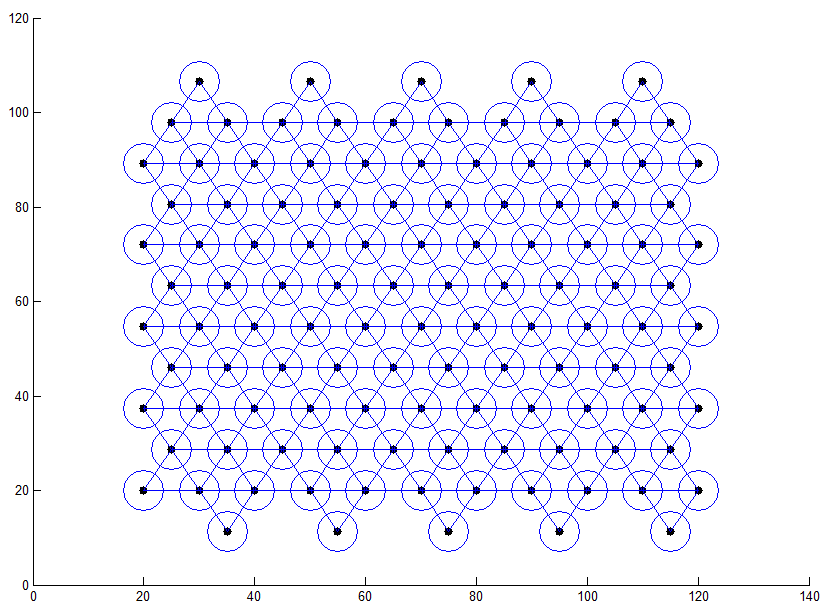
\includegraphics[width=10cm,height=7cm]{chapter5/figure5-1.png}
	\bicaption[fig:simulation_topo]{MATLAB平台下112个机器人构成的6邻居网络拓扑}{MATLAB平台下112个机器人构成的6邻居网络拓扑}{Fig}{The six-neighbor network topology constructed by 112 robots in MATLAB.}
\end{figure}

在仿真中,主要将本文所提算法与文献\parencite{张飞2008移动机器人覆盖问题的研究}中的无梯度分布情况下的自修复算法(下文称随机自修复算法)和文献\parencite{liu2015gradient}中的存在局部极小问题的自修复算法(下文称局部最优自修复算法)在相同的编队拓扑网络下进行比较。对算法的性能主要考察以下指标:\\
\indent 1)邻接矩阵的第二大特征值$\lambda_2$:由引理\ref{lem:lambda2}可知,邻接矩阵的第二大特征值$\lambda_2$可以用来衡量编队网络同步的稳定性和鲁棒性。$\lambda_2$越小,编队同步性能越好。此指标也是仿真中主要考察的一个指标。\\
\indent 2)修复机器人个数:修复机器人个数的多少代表着修复路径的长短,从而直接影响着编队自修复的效率,修复机器人个数越少,修复效率越高。\\
\indent 3)修复机器人总移动距离:此指标计算所有修复机器人在修复过程中移动距离的总和。之所以考察修复机器人的移动距离,是因为移动距离与能量消耗有关,在实际中具有重要意义。

\section{单个机器人丢失仿真对比}
首先进行单个机器人丢失的仿真对比。在相同的拓扑网络中使得同一个机器人丢失,分别应用不同的自修复算法进行自修复。图\ref{fig:random_single}描述了在由112个机器人构成的6邻居网络下进行的随机自修复仿真。坐标系内的所有实现圆点表示机器人的期望队形,每一个实心圆点对应一个机器人的期望位置。机器人中心的"x"表示机器人的当前位置。初始状态下,每一个机器人处在以期望位置为圆心,半径为5的范围内的一个随机位置,然后向期望位置移动,如图\ref{fig:random_single}(a)所示。当图\ref{fig:random_single}(b)中的空缺处出现机器人缺失时,根据文献\parencite{张飞2008移动机器人覆盖问题的研究}中的自修复规则选择一条修复路径,如图中红色机器人所示。修复机器人采用递归修复的方式一次填补对应的空缺,最终等效成一个度极小机器人修复缺失机器人。
\begin{figure*}[!htbp]
	\centering
	\begin{tabular}{cc}
	\subfigure[]{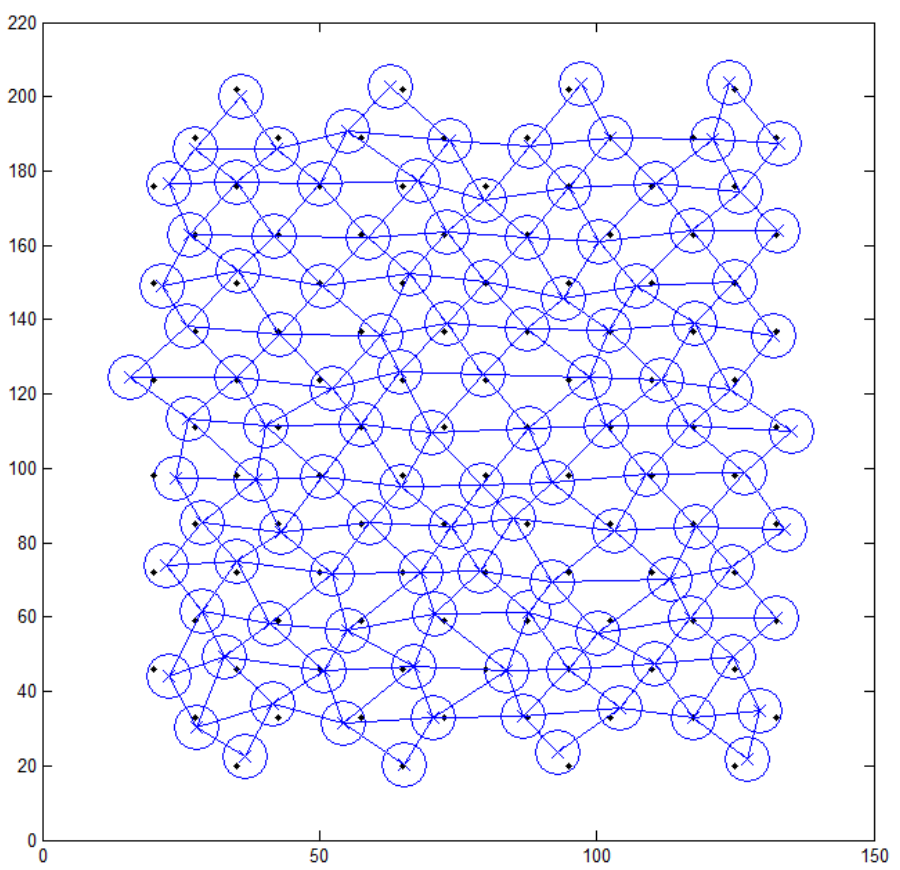
\includegraphics[width=6cm,height=6cm]{chapter5/Random_Single_a.png}} & 
	\hspace{1cm}
	\subfigure[]{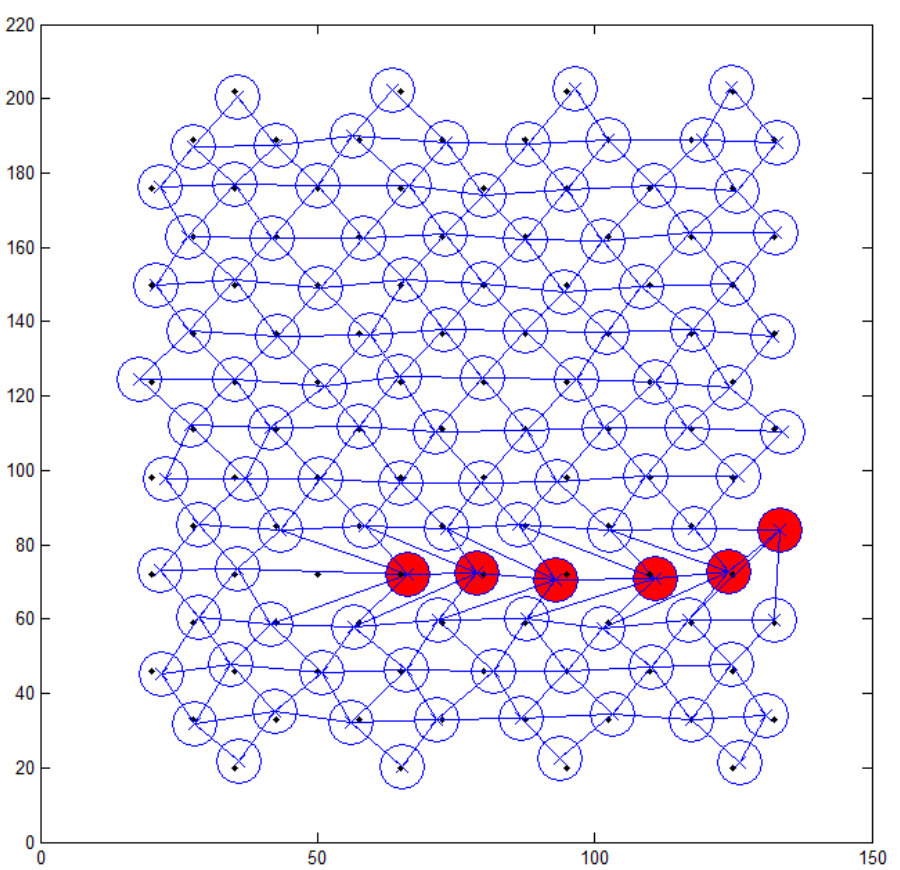
\includegraphics[width=6cm,height=6cm]{chapter5/Random_Single_b.png}} \\
	\subfigure[]{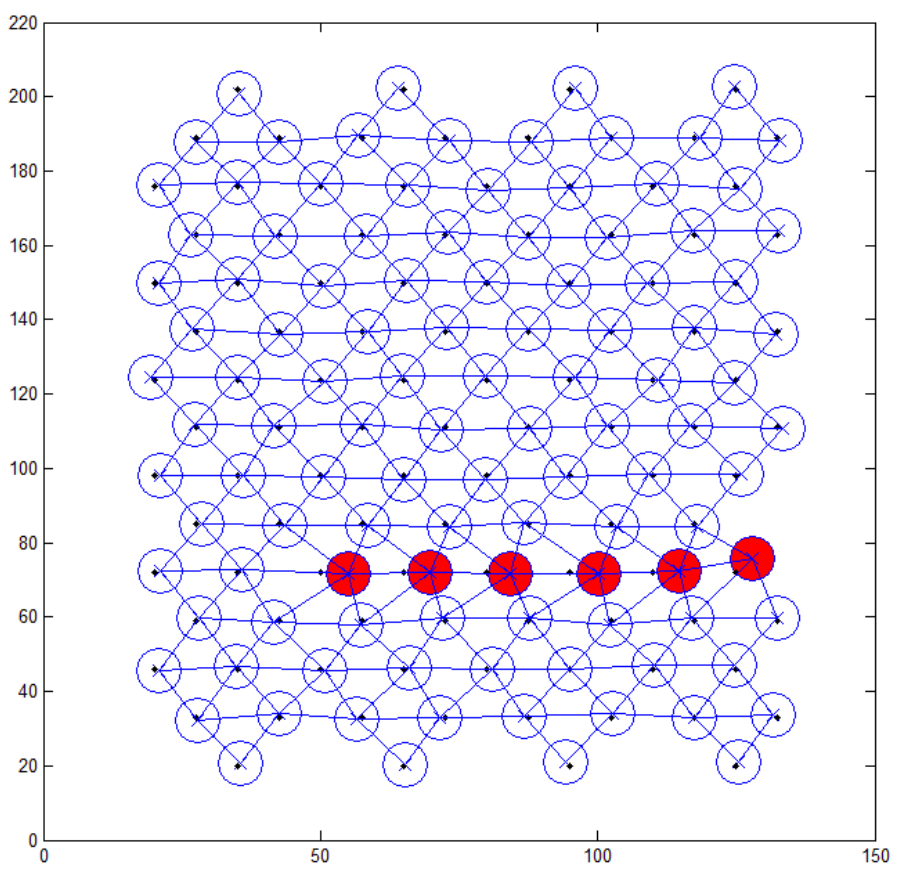
\includegraphics[width=6cm,height=6cm]{chapter5/Random_Single_c.png}} &
	\hspace{1cm}
	\subfigure[]{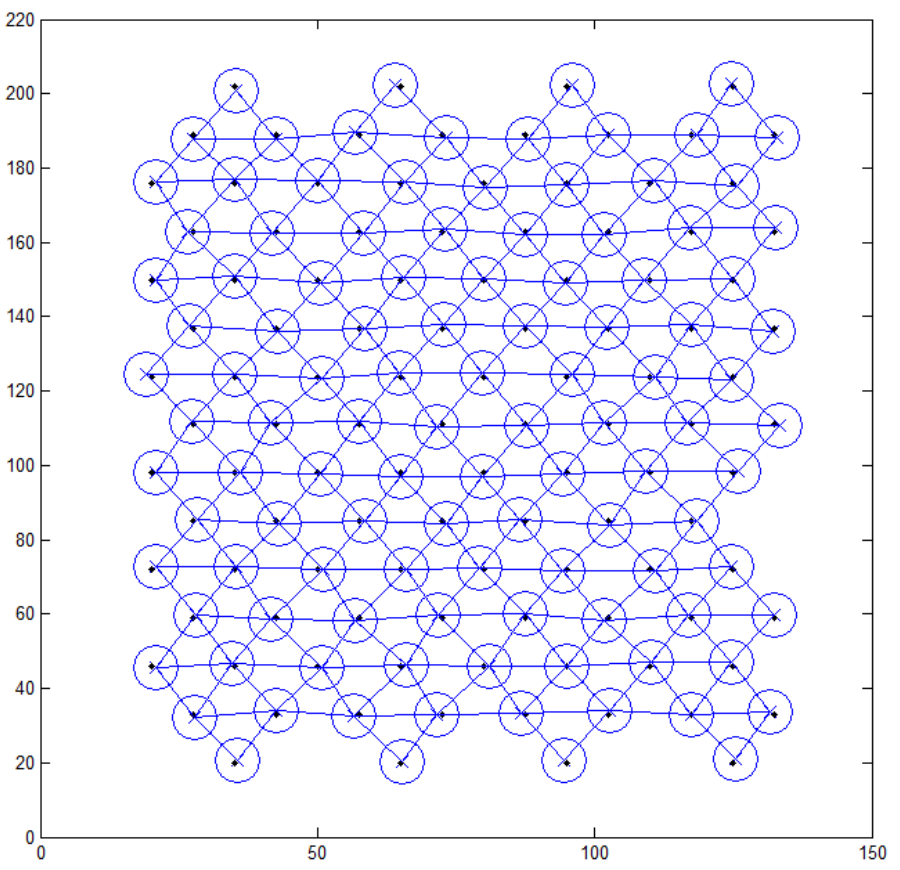
\includegraphics[width=6cm,height=6cm]{chapter5/Random_Single_d.png}}	
	\end{tabular}
	\bicaption[fig:random_single]{6邻居网络拓扑下随机自修复算法仿真过程}{6邻居网络拓扑下随机自修复算法仿真过程}{Fig}{The process of random self-healing algorithm simulation for six neighbor network.}
\end{figure*}

由于随机自修复算法中只根据机器人度的信息进行判断,当多个满足条件的机器人度相同的时候,随机选择修复机器人。因此修复路径的随机性很大,可以看出图\ref{fig:random_single}中的修复路径并不是最短的,且存在局部极小问题。图\ref{fig:random_RepairingPath}中分别为仿真中其他几种修复路径。
\begin{figure*}[!htbp]
	\centering
	\begin{tabular}{cc}
		\subfigure[]{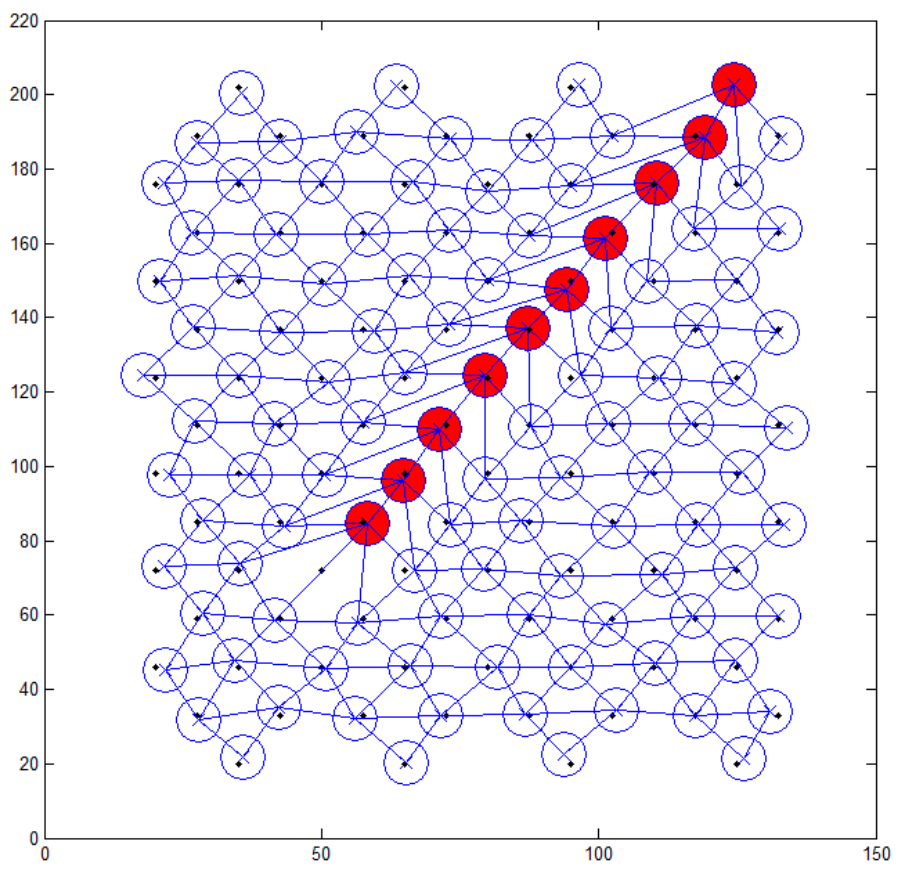
\includegraphics[width=6cm,height=6cm]{chapter5/figure5-3a.png}} &
		\hspace{1cm}
		\subfigure[]{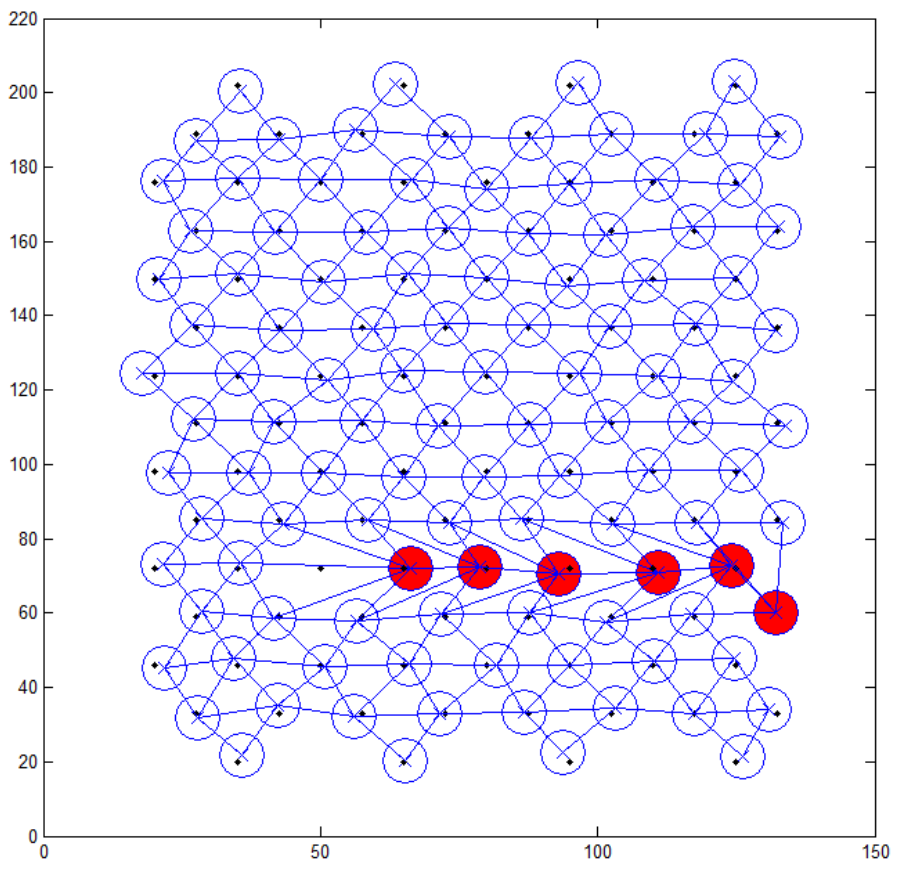
\includegraphics[width=6cm,height=6cm]{chapter5/figure5-3b.png}} \\
		\subfigure[]{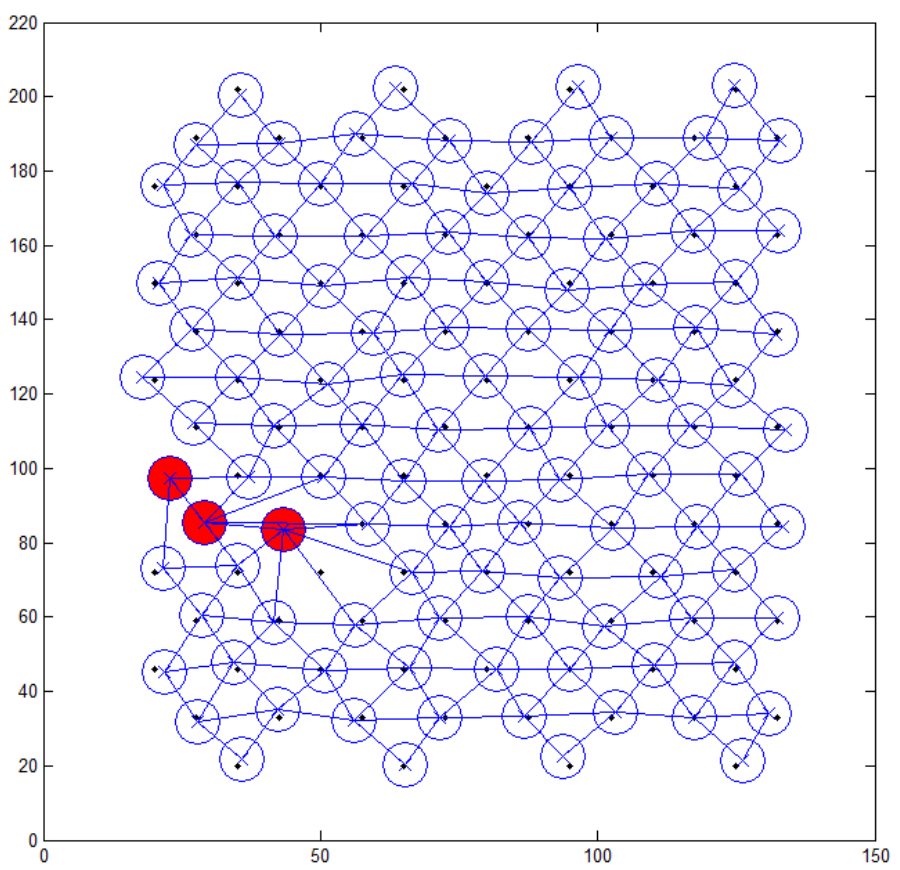
\includegraphics[width=6cm,height=6cm]{chapter5/figure5-3c.png}} &
		\hspace{1cm}
		\subfigure[]{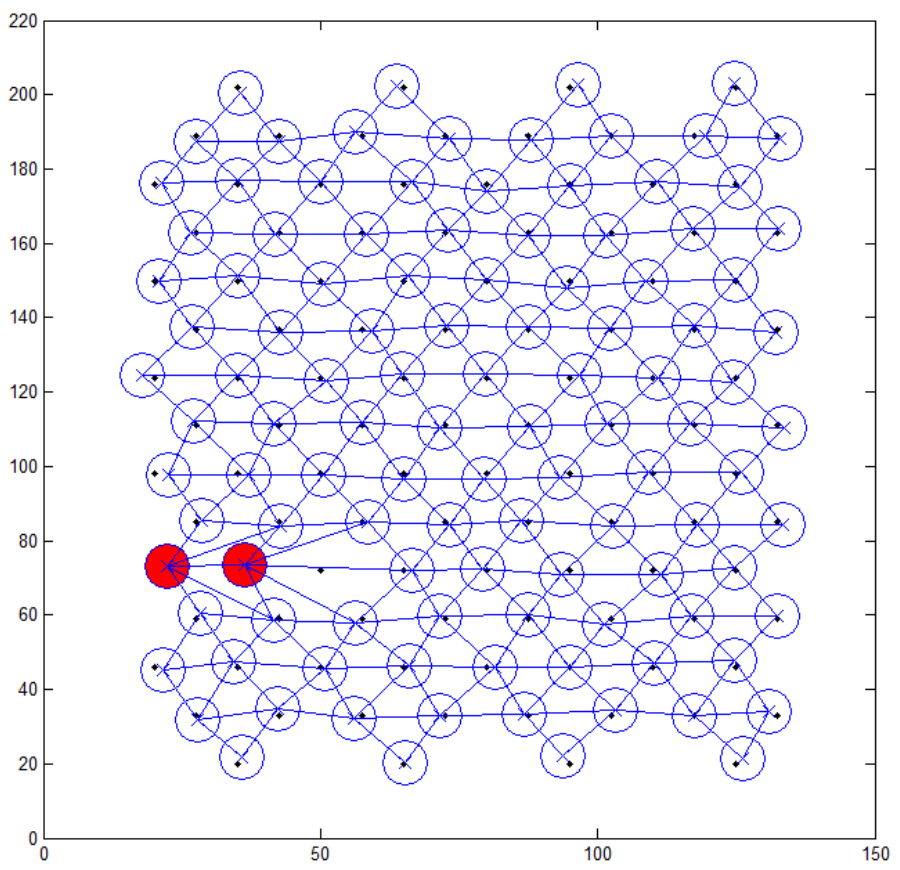
\includegraphics[width=6cm,height=6cm]{chapter5/figure5-3d.png}}
	\end{tabular}
	\bicaption[fig:random_RepairingPath]{随机自修复仿真中几种不同的修复路径}{随机自修复仿真中几种不同的修复路径}{Fig}{Several repairing paths for random self-healing algorithm.}
\end{figure*}

在文献\parencite{liu2015gradient}中引入了梯度信息,仿真过程如图\ref{fig:local_single}所示。代表机器人的圆圈中填充的颜色深浅表示梯度值的大小,颜色越深,梯度值越小,黑色表示梯度源节点。同样,空缺表示缺失机器人,图\ref{}(b)中缺失机器人与随机自修复仿真中的缺失机器人相同。红色圆圈代表修复机器人。由于引入梯度,因此算法降低了随机性,每次都能找到一条最短的修复路径。但是从仿真中也可以看出,算法存在的局部极小问题,仿真中最后的修复机器人度为3,而全局度最小的机器人度为2。因此同步性改善并不是最优的。
\begin{figure*}[!htbp]
	\centering
	\begin{tabular}{cc}
		\subfigure[]{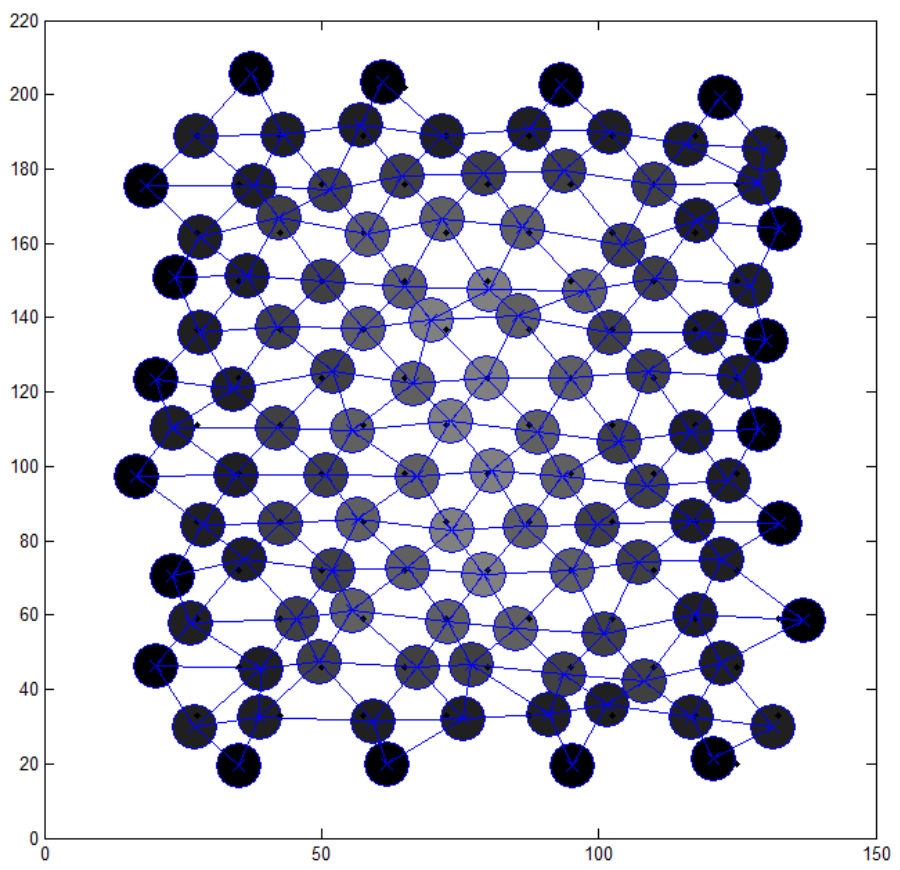
\includegraphics[width=6cm,height=6cm]{chapter5/figure5-4a.png}} &
		\hspace{1cm}
		\subfigure[]{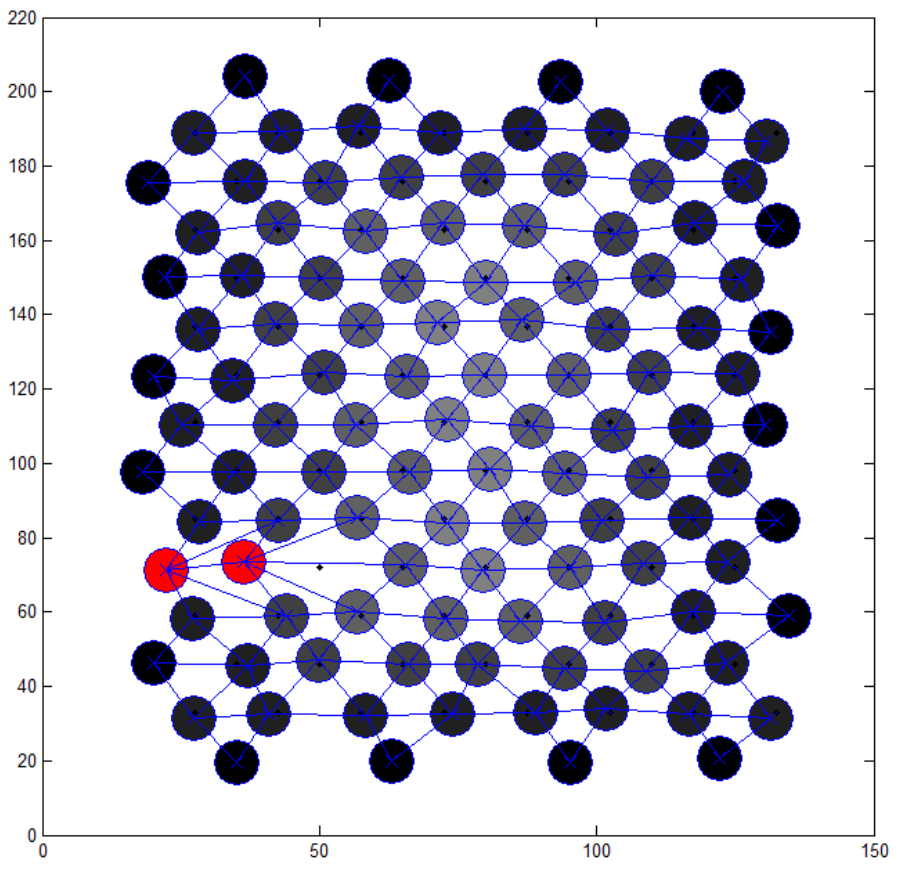
\includegraphics[width=6cm,height=6cm]{chapter5/figure5-4b.png}} \\
		\subfigure[]{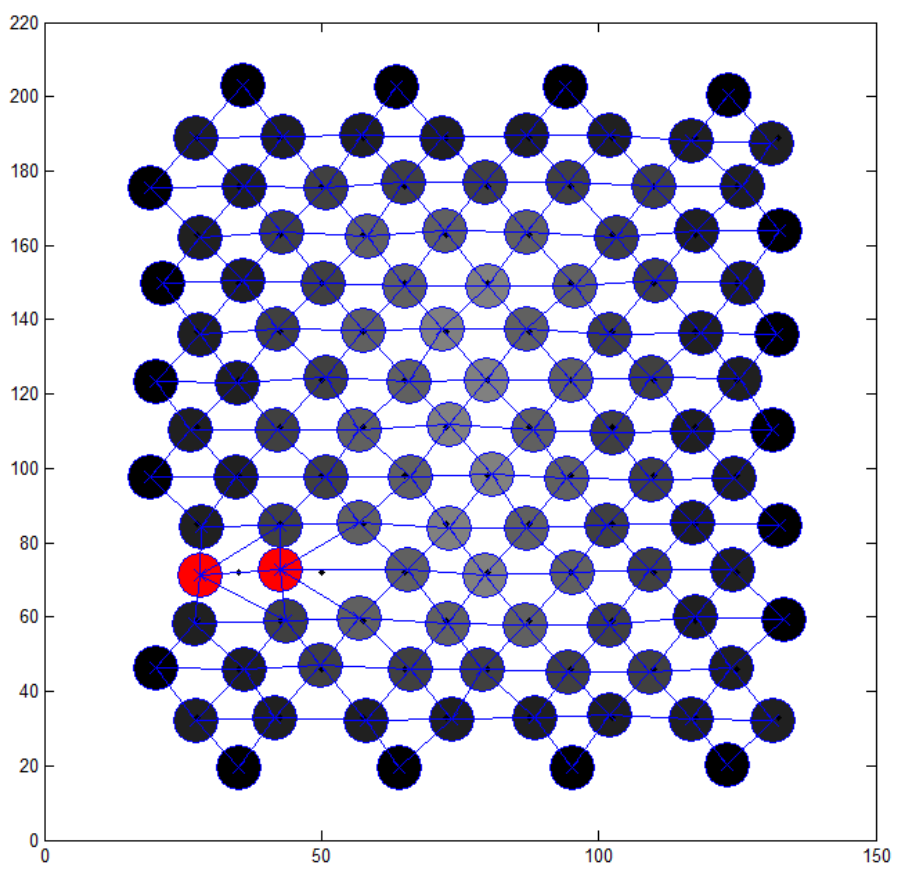
\includegraphics[width=6cm,height=6cm]{chapter5/figure5-4c.png}} &
		\hspace{1cm}
		\subfigure[]{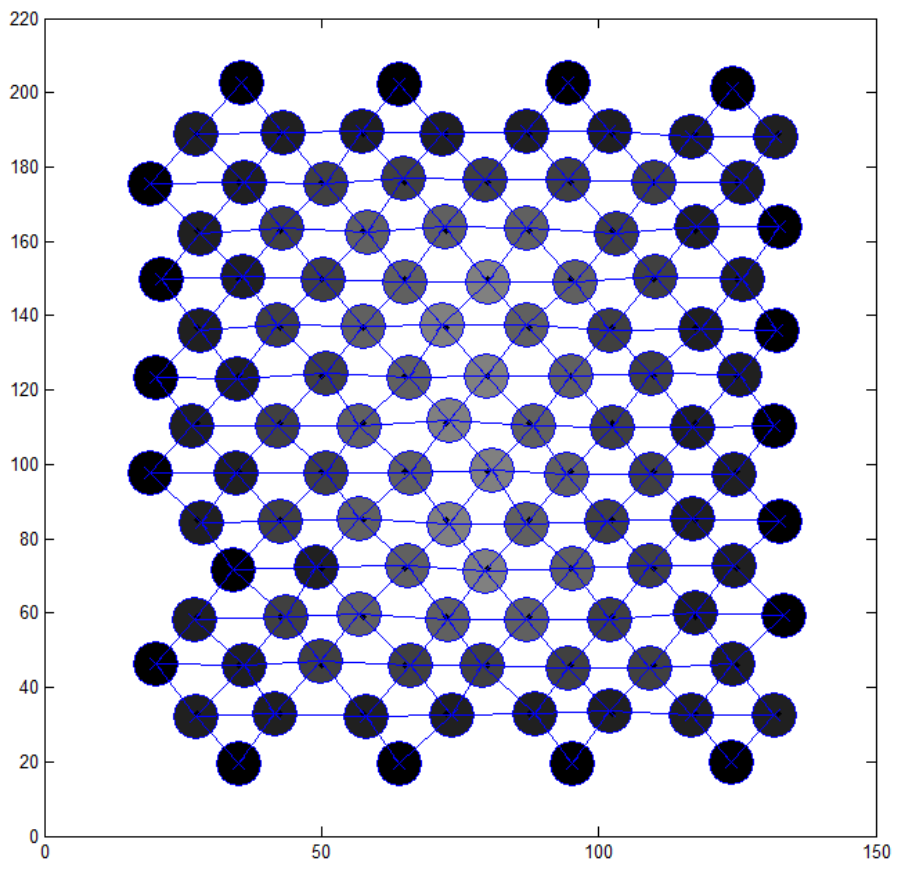
\includegraphics[width=6cm,height=6cm]{chapter5/figure5-4d.png}}
	\end{tabular}
	\bicaption[fig:local_single]{6邻居网络拓扑下局部最优自修复算法仿真过程}{6邻居网络拓扑下局部最优自修复算法仿真过程}{Fig}{The process of local optimal self-healing algorithm simulation for six neighbor network.}
\end{figure*}

本文算法就是为避免以上问题,从而实现同步性改善全局最优而设计。通过改善梯度扩散的方式而避免局部极小问题。图\ref{fig:global_single}是本文的同步性改善全局最优的自修复算法仿真过程。从图\ref{fig:global_single}(a)中可以看出,本文算法最终形成的稳定梯度分布形式与文献\parencite{liu2015gradient}中的不同,在图\ref{fig:local_single}(a)中的那些度为3的梯度源节点被更新,不再是梯度源节点。当出现缺失机器人时,缺失机器人的邻居检测到缺失后,自身状态转移到候选修复状态进行竞选。竞选成功的机器人转移到修复状态,然后继续选择下一步修复机器人将修复状态传递下去,直到梯度源节点从而选出一条修复路径如图\ref{fig:global_single}(c)所示。修复完成后的网络拓扑如图\ref{fig:global_single}(d)所示。

\begin{figure*}[!htbp]
	\centering
	\begin{tabular}{cc}
		\subfigure[]{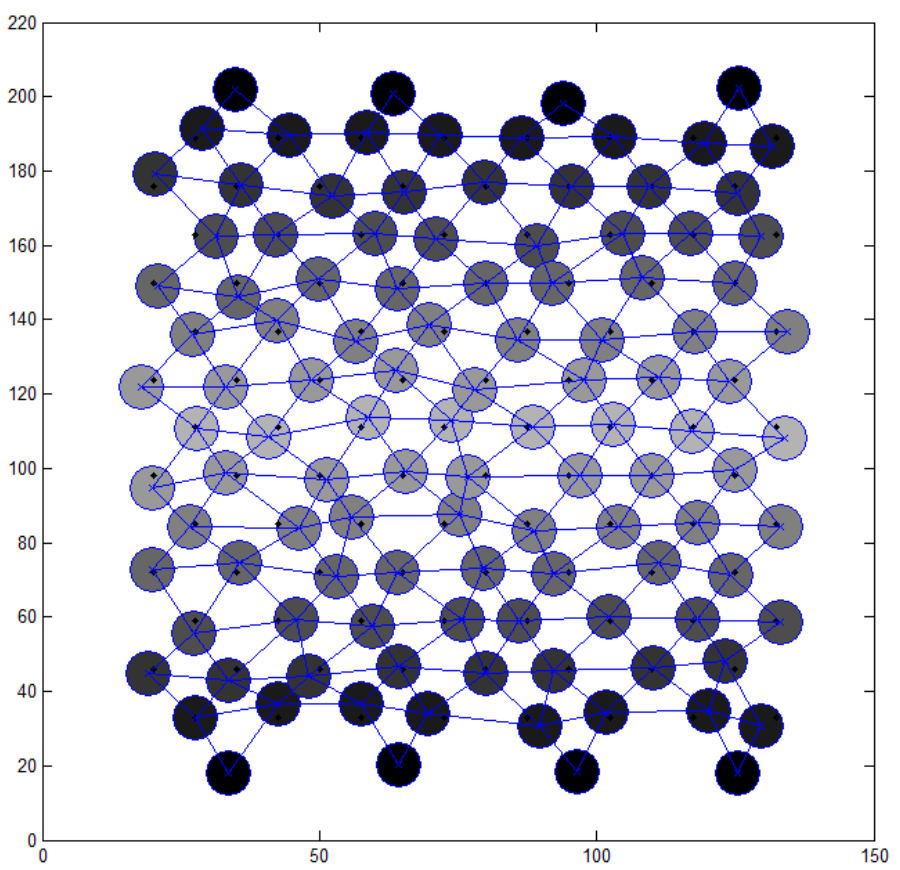
\includegraphics[width=6cm,height=6cm]{chapter5/figure5-5a.png}} &
		\hspace{1cm}
		\subfigure[]{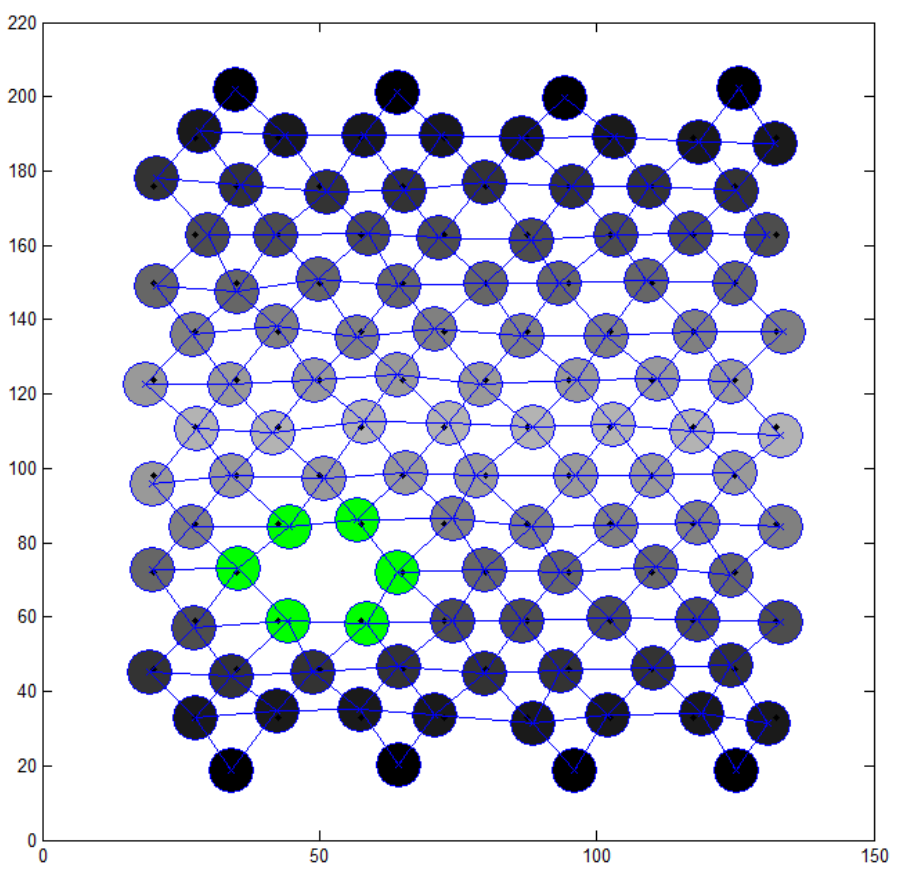
\includegraphics[width=6cm,height=6cm]{chapter5/figure5-5b.png}} \\
		\subfigure[]{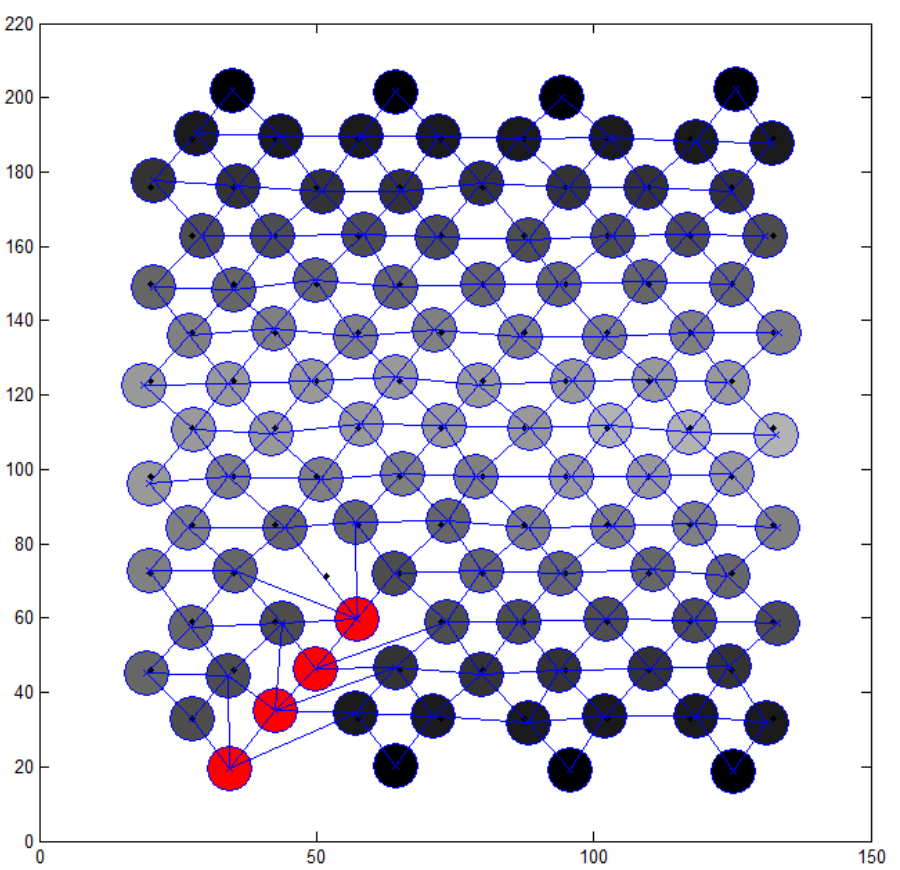
\includegraphics[width=6cm,height=6cm]{chapter5/figure5-5c.png}} &
		\hspace{1cm}
		\subfigure[]{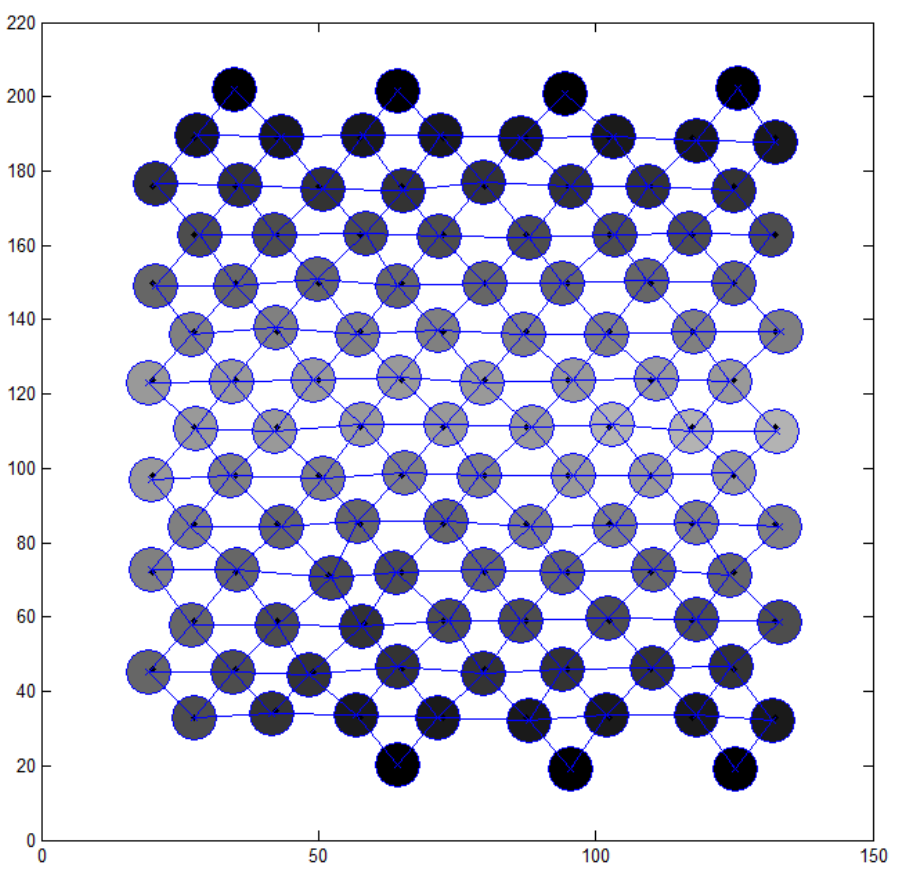
\includegraphics[width=6cm,height=6cm]{chapter5/figure5-5d.png}}
	\end{tabular}
	\bicaption[fig:global_single]{6邻居网络拓扑下全局最优自修复算法仿真过程}{6邻居网络拓扑下全局最优自修复算法仿真过程}{Fig}{The process of global optimal self-healing algorithm simulation for six neighbor network.}
\end{figure*}

在仿真中针对第二大特征值,修复机器人个数,修复机器人总移动距离三个指标将三种自修复算法进行了对比。图\ref{fig:simulation_result}是仿真结果的对比分析。在仿真中对同一个丢失机器人进行了十次重复试验,横坐标的实验ID表示$1~10$次实验。从图\ref{fig:simulation_result}(a)中可以看出,10次实验本文算法均取得了最小的第二大特征值,即意味着本文算法均获得了最优的同步性改善效果,且是稳定的。局部最优自修复算法虽然也是稳定的,但是由于产生了局部极小,因此无法取得最优的同步性改善效果。随机自修复算法由于存在过多的随机性,因此每一次的结果都无法保证相同,是不稳定的。对于修复机器人个数与修复机器人移动距离同样本文算法与局部最优自修复算法是稳定的,随机自修复算法不稳定。在修复机器人个数与修复机器人总移动距离的对比上,局部最优自修复算法当在产生局部极小问题时可能会获得比本文算法获得更少的修复机器人个数与总移动距离。但是根据前文3.4.3节有关修复时间的分析,虽然本文算法相比局部最优自修复算法具有更多的修复机器人个数与总移动距离,但是这并不会增加修复时间,因此对自修复的时间效率影响不大。
\begin{figure*}[!htbp]
	\centering
	\begin{tabular}{cc}
		\subfigure[第二大特征值对比结果]{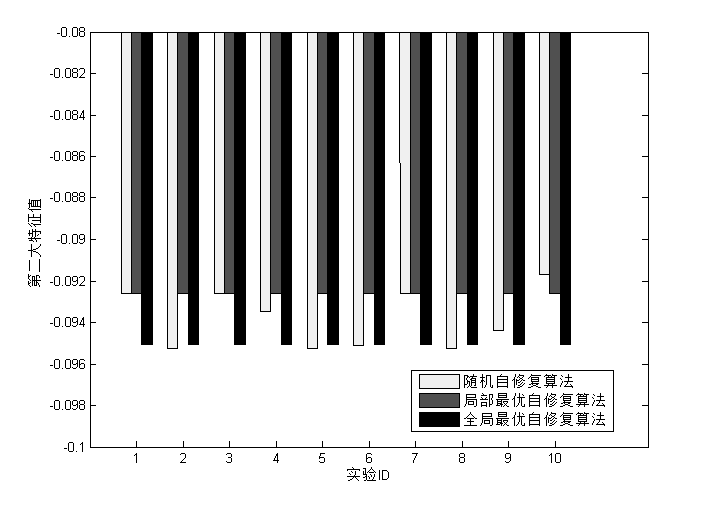
\includegraphics[width=8cm,height=6cm]{chapter5/figure5-6a.png}} 
		\subfigure[修复机器人个数对比结果]{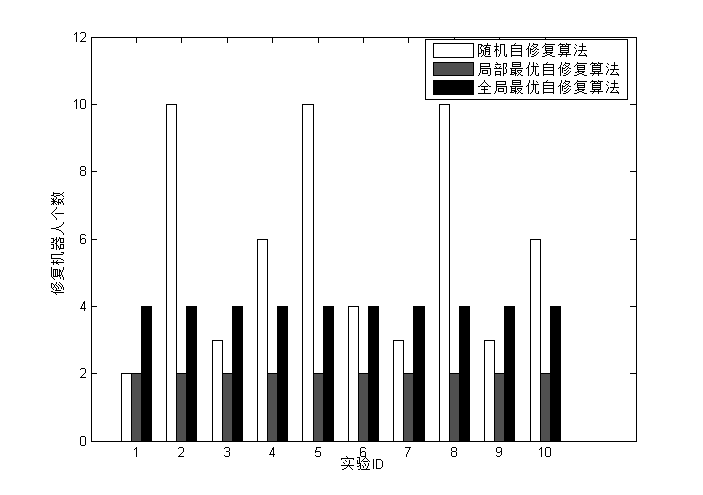
\includegraphics[width=8cm,height=6cm]{chapter5/figure5-6b.png}} \\
		\subfigure[修复机器人总移动距离对比结果]{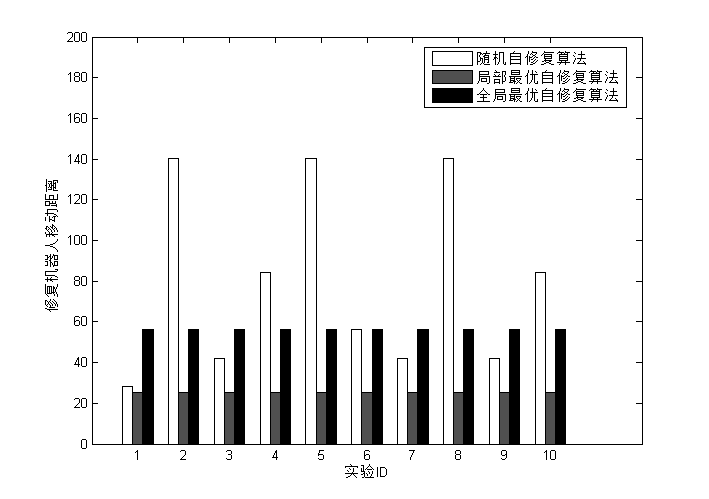
\includegraphics[width=8cm,height=6cm]{chapter5/figure5-6c.png}}
	\end{tabular}
	\bicaption[fig:simulation_result]{三种自修复算法仿真结果对比}{三种自修复算法仿真结果对比}{Fig}{The comparation of simulation result among three self-healing algorithm.}
\end{figure*}

\section{多个机器人丢失仿真对比}
虽然单个机器人丢失的情况验证了本文算法的有效性和可行性,但是实际情况中可能存在不止一个机器人丢失的情况。这些丢失机器人可能相互独立,可能互为邻居。然而我们假设丢失的机器人至少有一个邻居依然存在编队网络中。因为本文算法是完全分布式实现的,机器人只能和邻居通信,也只有机器人的邻居能够感知到它的存在于丢失。因此如果丢失的机器人所有邻居也全部丢失,则没有机器人能够感知到它的丢失,修复也就无法进行了。

图\ref{fig:random_multi}是在多机器人丢失的情况下应用随机自修复算法进行自修复所选择的修复路径。图中分别对应丢失2个,3个,4个,5个机器人时的修复路径。由于随机自修复算法随机性比较大,因此这是每种情况下的一次修复路径选择。
\begin{figure*}[!htbp]
	\centering
	\begin{tabular}{cc}
		\subfigure[丢失两个机器人]{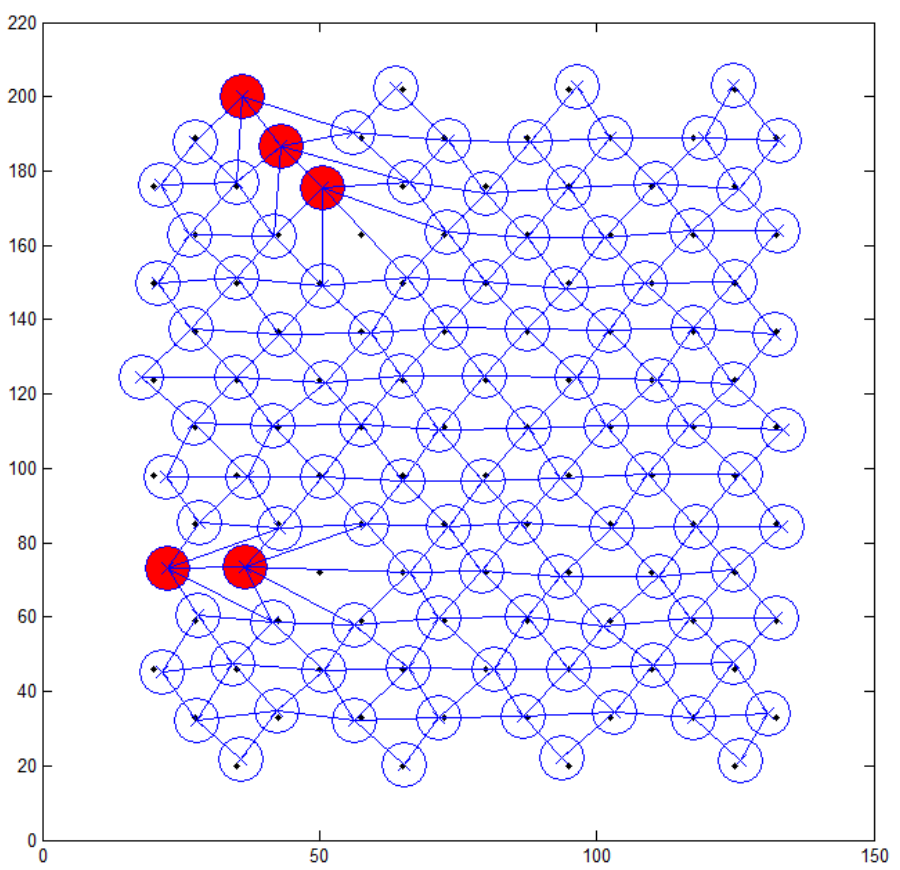
\includegraphics[width=6cm,height=6cm]{chapter5/figure5-7a.png}} &
		\hspace{1cm}
		\subfigure[丢失三个机器人]{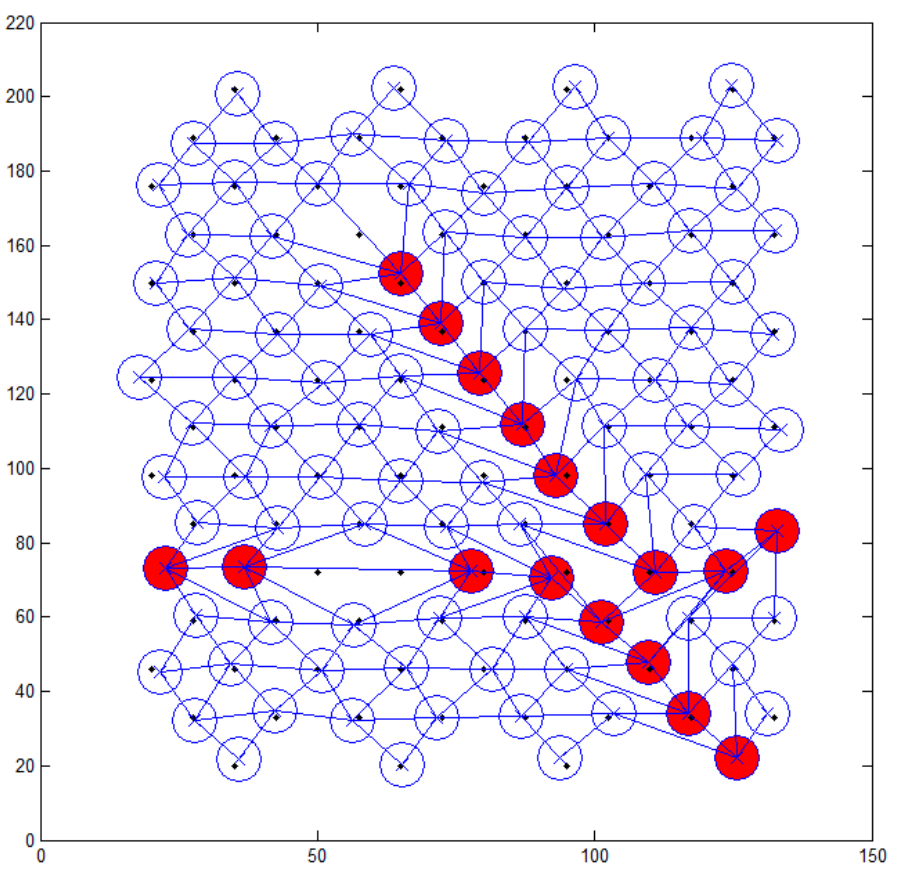
\includegraphics[width=6cm,height=6cm]{chapter5/figure5-7b.png}} \\
		\subfigure[丢失四个机器人]{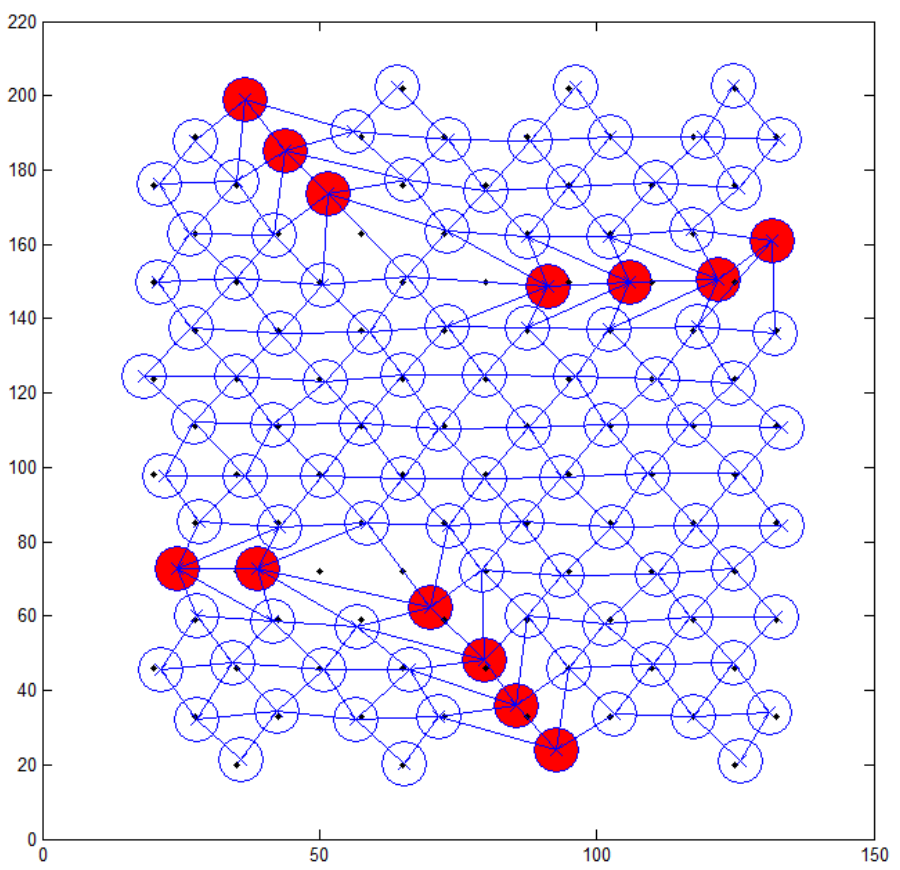
\includegraphics[width=6cm,height=6cm]{chapter5/figure5-7c.png}} &
		\hspace{1cm}
		\subfigure[丢失五个机器人]{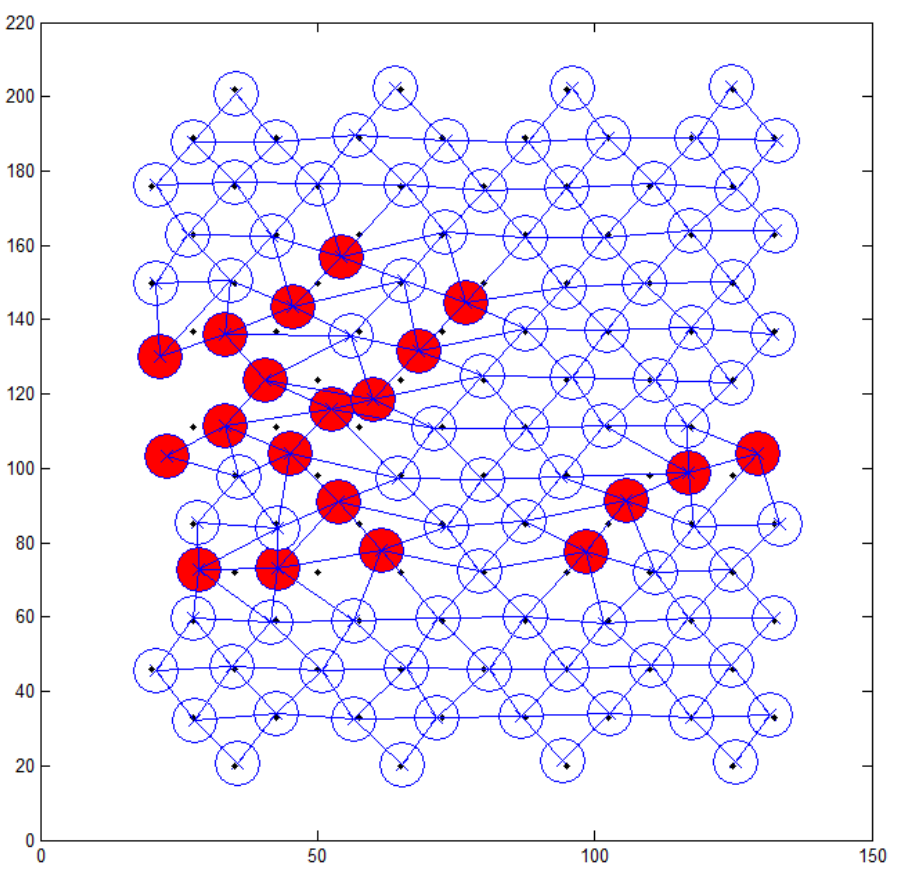
\includegraphics[width=6cm,height=6cm]{chapter5/figure5-7d.png}}	
	\end{tabular}
	\bicaption[fig:random_multi]{随机自修复算法针对多个丢失机器人的修复路径选择}{随机自修复算法针对多个丢失机器人的修复路径选择}{Fig}{The repairing paths of random self-healing algorithm for multiple failed robots.}
\end{figure*}

由于随机性的原因,某些修复路径包含的修复机器人会很多,这样就会导致多个机器人丢失后,整个编队过多机器人参与修复过程,这无论从编队的任务执行效率还是能量的消耗等方面都会造成不理的影响。而且在图\ref{fig:random_multi}(d)中由于3条修复路径使用两个度极小机器人,因此导致一条修复路径的最后一个修复机器人的空缺位置没有一个度极小机器人来填补,造成修复不完全的问题。这都是在随机自修复算法下会产生的问题。

图\ref{fig:local_multi}是在多机器人丢失的情况下应用局部最优自修复算法进行自修复所选择的修复路径。可以看到在引入梯度后多个丢失机器人的修复路径不会冲突,所以不会造成修复不完全的问题。同时还能够相对减少修复机器人的个数。

\begin{figure*}[!h]
	\centering
	\begin{tabular}{cc}
		\subfigure[丢失两个机器人]{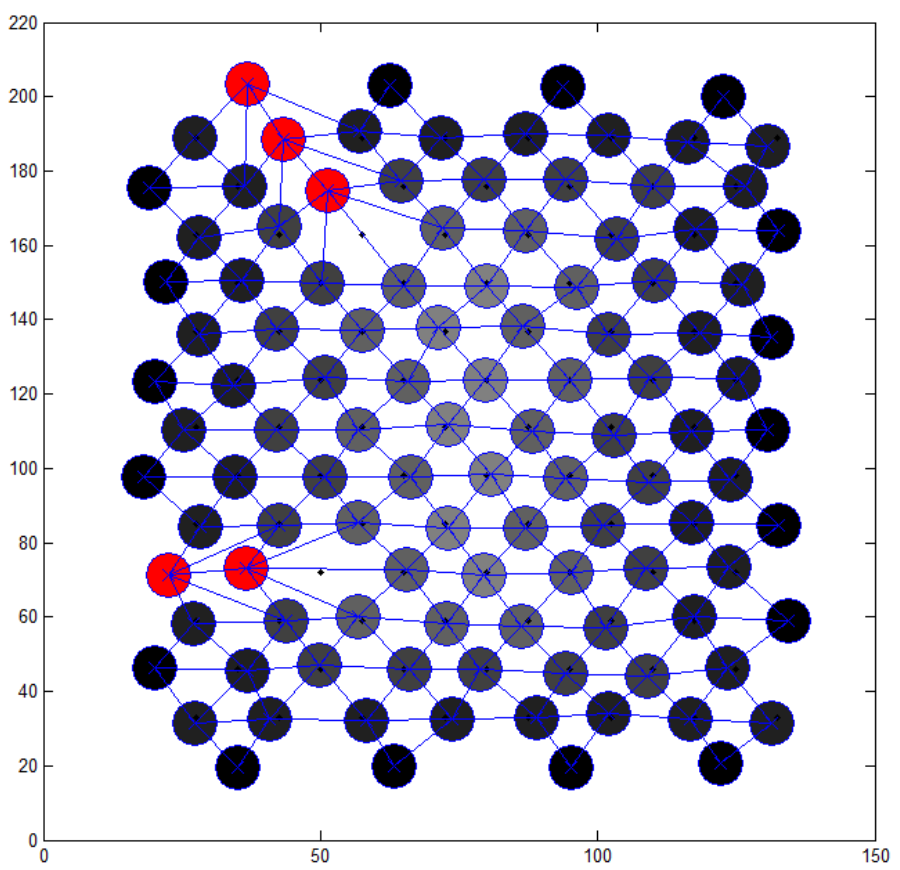
\includegraphics[width=6cm,height=6cm]{chapter5/figure5-8a.png}} &
		\hspace{1cm}
		\subfigure[丢失三个机器人]{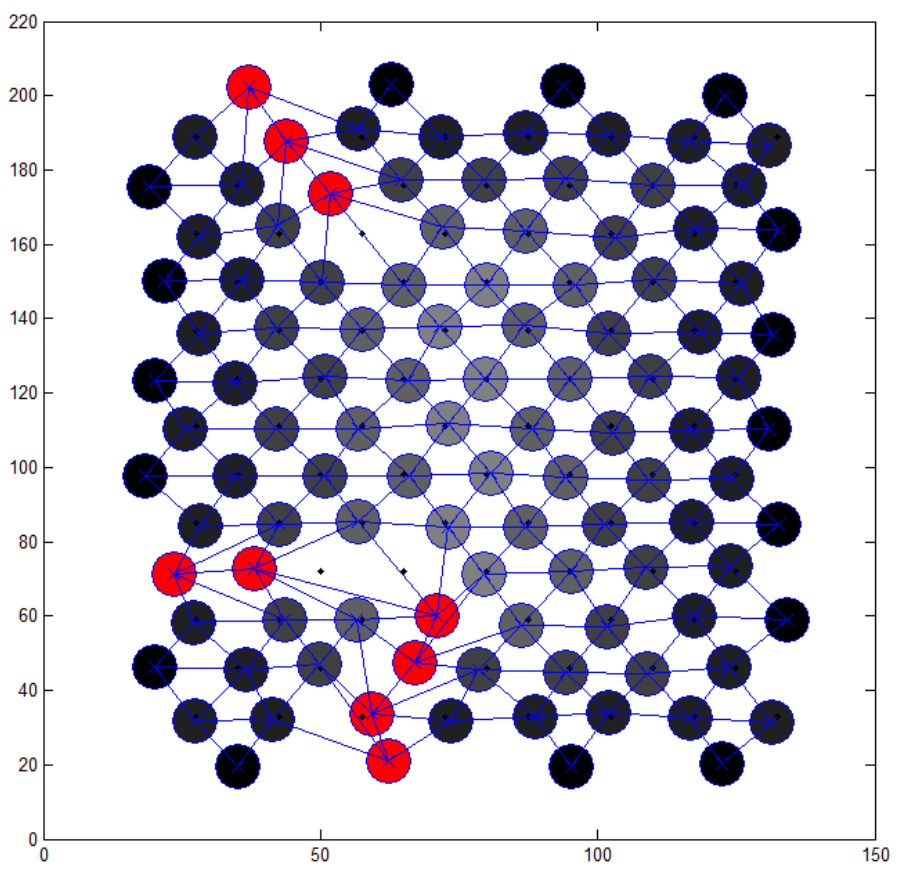
\includegraphics[width=6cm,height=6cm]{chapter5/figure5-8b.png}} \\
		\subfigure[丢失四个机器人]{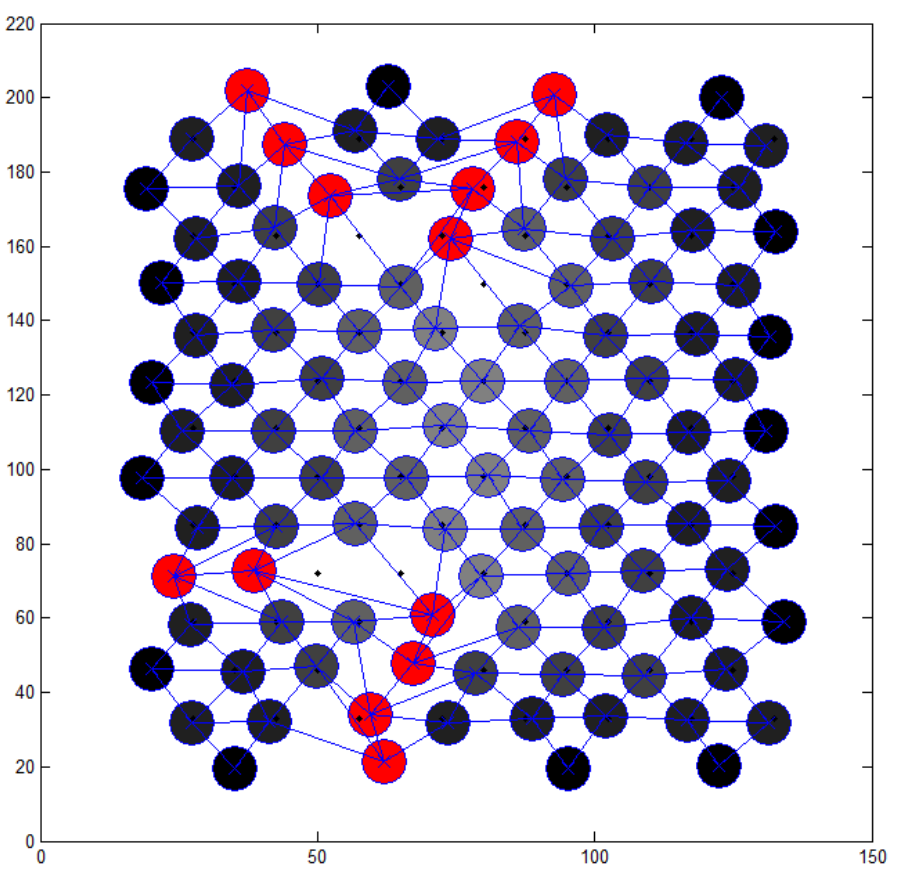
\includegraphics[width=6cm,height=6cm]{chapter5/figure5-8c.png}} &
		\hspace{1cm}
		\subfigure[丢失五个机器人]{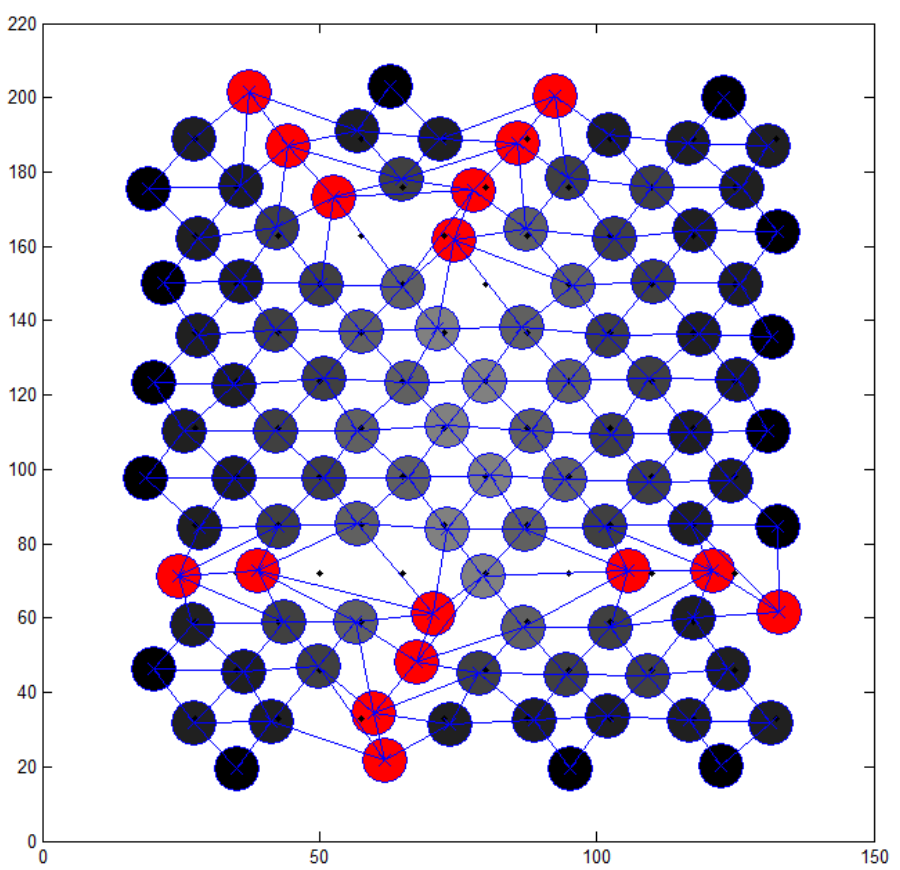
\includegraphics[width=6cm,height=6cm]{chapter5/figure5-8d.png}}
	\end{tabular}
	\bicaption[fig:local_multi]{局部最优自修复算法针对多个丢失机器人的修复路径选择}{局部最优自修复算法针对多个丢失机器人的修复路径选择}{Fig}{The repairing paths of local optimal self-healing algorithm for multiple failed robots.}
\end{figure*}
	
局部最优自修复算法的目的主要是在改善编队同步性过程中实现修复路径的最短,因此在牺牲了同步性改善效果之后针对每一个丢失机器人应该用最短的修复路径进行修复,然而在某些情况下该算法无法达到修复路径最短。当两个丢失机器人互为邻居时,可能会造成一个丢失机器人的最短修复路径包含另一个丢失机器人,如图\ref{fig:local_multi}(c)所示。此时就无法保证这个丢失机器人的修复路径最短。

图\ref{fig:global_multi}是在多机器人丢失的情况下应用全局最优自修复算法进行自修复所选择的修复路径。根据本文的梯度扩散规则以及自修复算法,每一个丢失机器人都可以最终等效成由编队中度最小机器人修复。根据引理\ref{lem:degree_syn},可以实现编队同步性改善全局最优。
\begin{figure*}[]
	\centering
	\begin{tabular}{cc}
		\subfigure[丢失两个机器人]{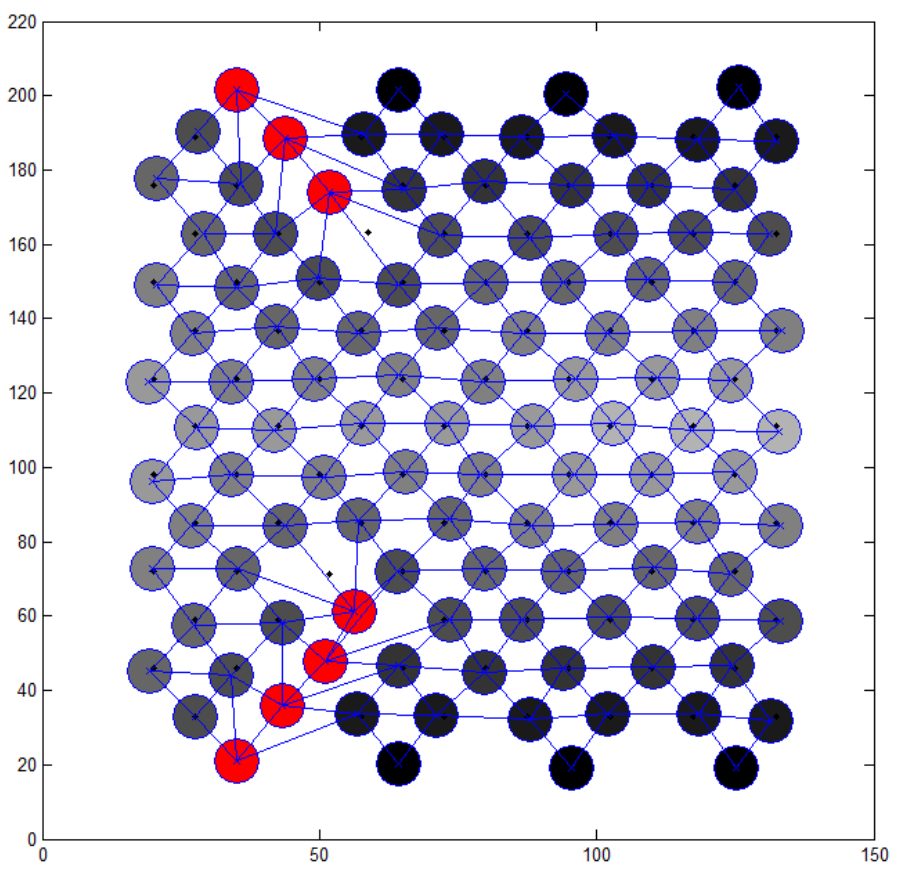
\includegraphics[width=6cm,height=6cm]{chapter5/figure5-9a.png}} &
		\hspace{1cm}
		\subfigure[丢失三个机器人]{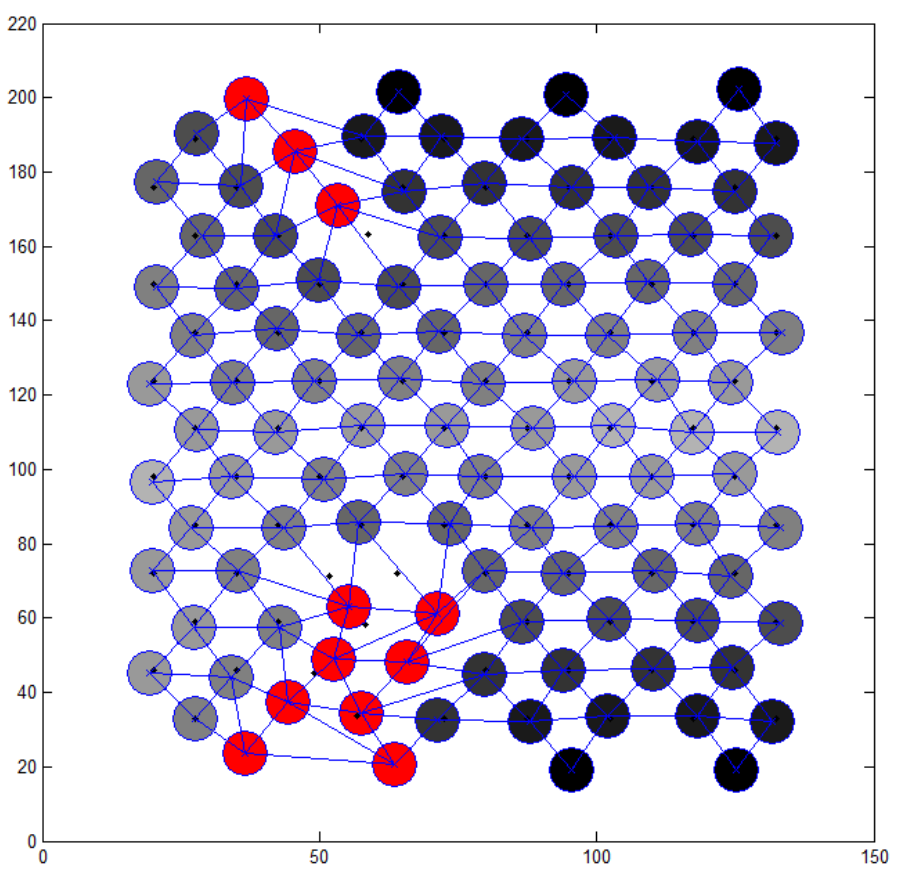
\includegraphics[width=6cm,height=6cm]{chapter5/figure5-9b.png}} \\
		\subfigure[丢失四个机器人]{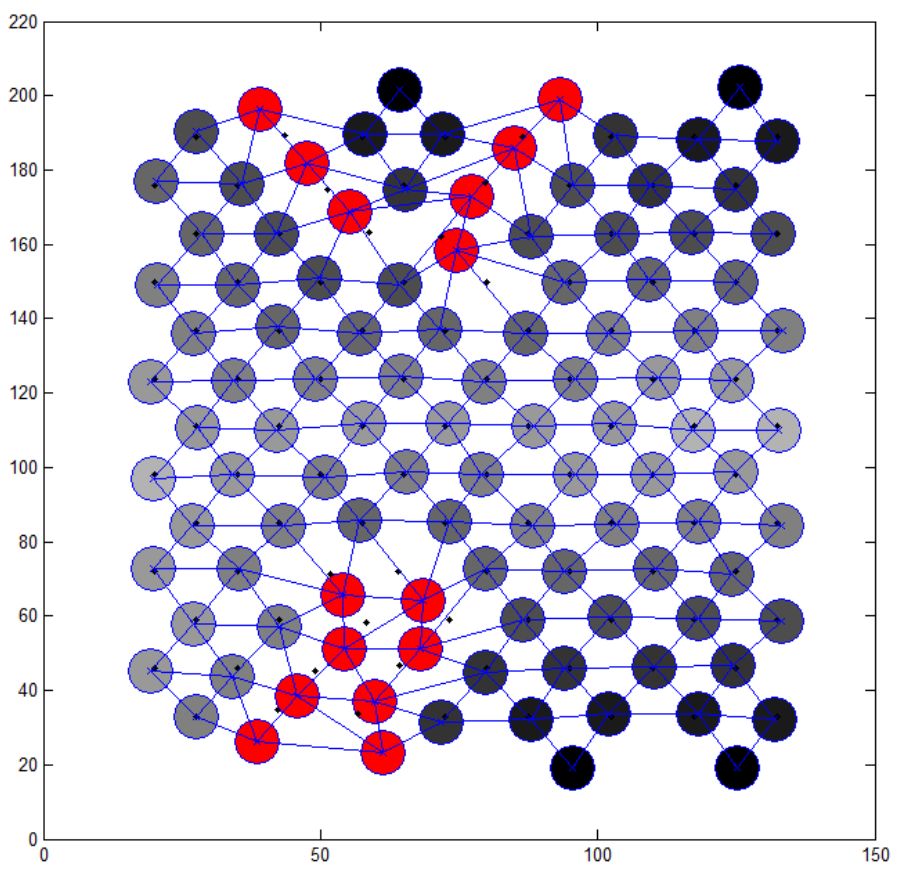
\includegraphics[width=6cm,height=6cm]{chapter5/figure5-9c.png}} &
		\hspace{1cm}
		\subfigure[丢失五个机器人]{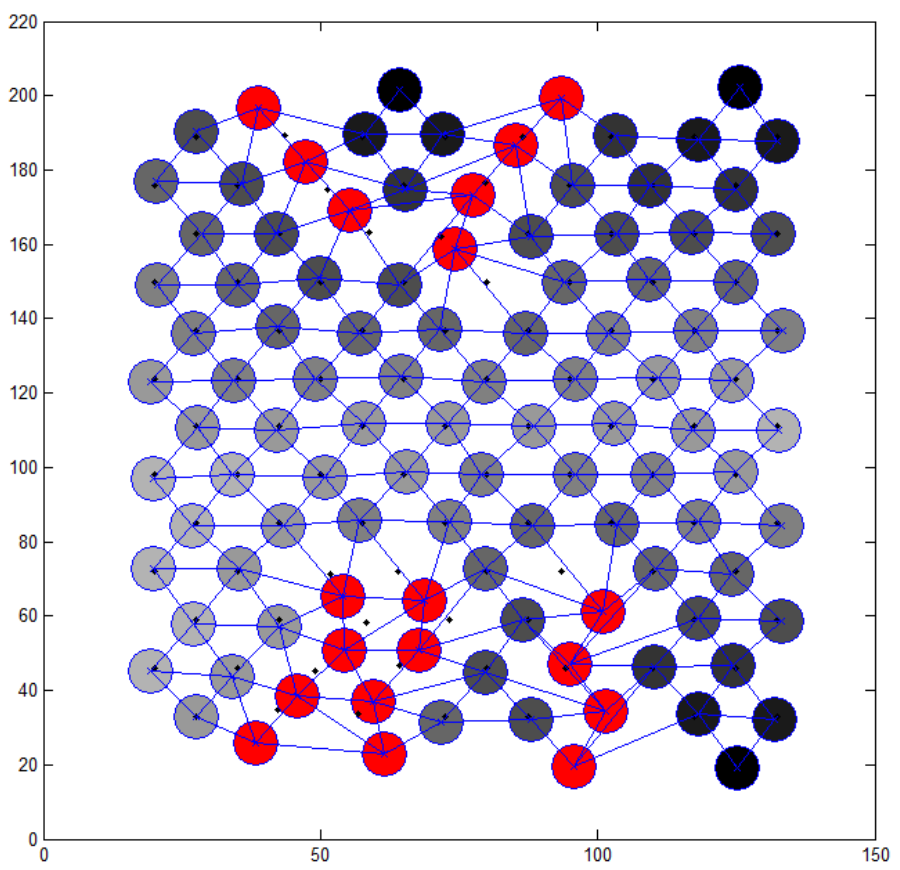
\includegraphics[width=6cm,height=6cm]{chapter5/figure5-9d.png}}
	\end{tabular}
	\bicaption[fig:global_multi]{全局最优自修复算法针对多个丢失机器人的修复路径选择}{全局最优自修复算法针对多个丢失机器人的修复路径选择}{Fig}{The repairing paths of global optimal self-healing algorithm for multiple failed robots.}
\end{figure*}

图\ref{fig:multi_result}是3种算法应用在多个丢失机器人情况下的指标对比结果。仿真中分别针对丢失2、3、4、5个机器人的情况做10次重复试验,最终计算平均值,并记录最大最小值。从仿真结果可以看出,相比另两种算法本文算法具有最小的第二大特征值,即同步性改善效果最好。在修复机器人个数与修复机器人总移动距离上的仿真结果上局部最优自修复算法要略优于本文算法,主要是由于局部极小的问题,也因此使得同步性改善效果有限。根据每种情况下的10次重复试验结果可知,局部最优自修复算法与本文算法都是稳定的。另外从图\ref{fig:multi_result}(a)可知,在使用本文算法进行自修复的情况下,随着丢失机器人个数的增多,第二大特征值减小,同步性增强。这正好印证了文献\parencite{张飞2008移动机器人覆盖问题的研究}中所指出的机器人缺失对编队同步性的影响程度大小与缺失机器人的度以及缺失机器人数量的关系。即如图\ref{fig:sec_eigenvalue and failure ratio}所描述的关系,网络同步性随着编队网络中度最低机器人的缺失数量的增加而提高。
\begin{figure*}[!htbp]
	\centering
	\begin{tabular}{cc}
		\subfigure[第二大特征值仿真结果对比]{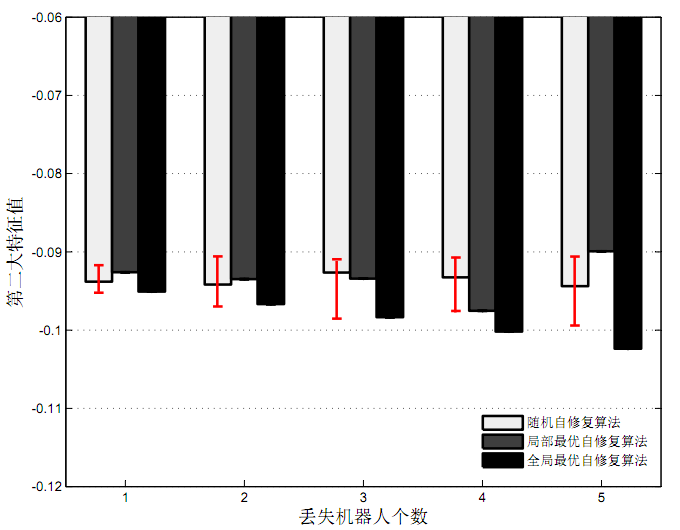
\includegraphics[width=7cm,height=6cm]{chapter5/figure5-10a.png}} 
		\hspace{1cm}
		\subfigure[修复机器人个数仿真结果对比]{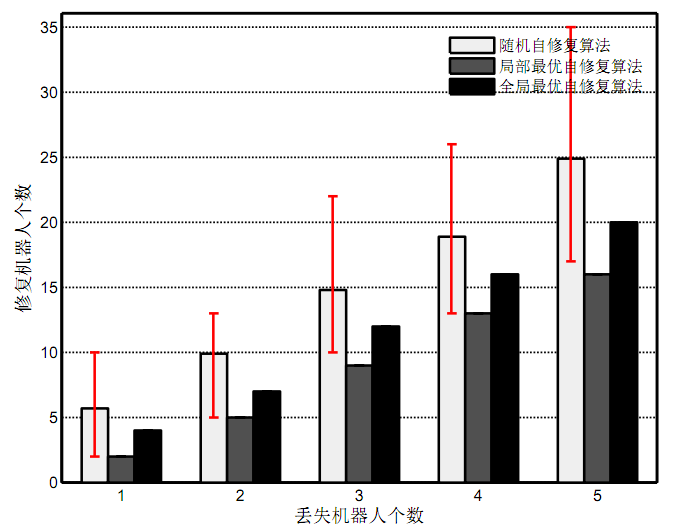
\includegraphics[width=7cm,height=6cm]{chapter5/figure5-10b.png}} \\
		\subfigure[修复机器人总移动距离仿真结果对比]{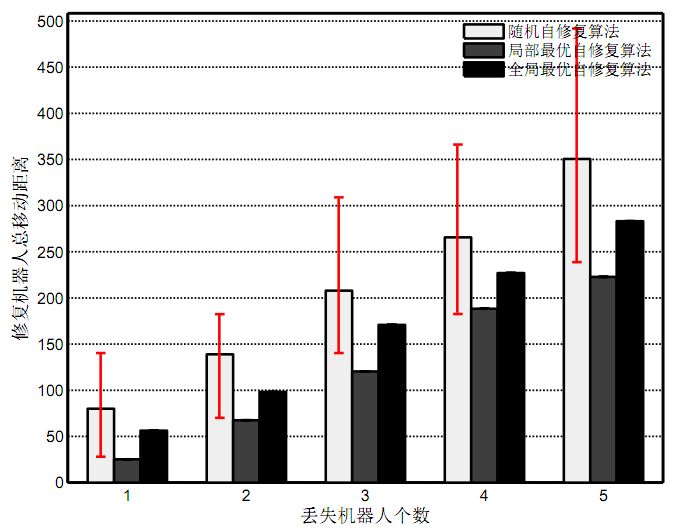
\includegraphics[width=7cm,height=6cm]{chapter5/figure5-10c.png}}
	\end{tabular}
	\bicaption[fig:multi_result]{多个丢失机器人仿真结果对比}{多个丢失机器人仿真结果对比}{Fig}{The comparation of simulation result for multiple failed robots.}
\end{figure*}

以上多个丢失机器人全部都是处在非梯度源节点的状态,然而,如果机器人的运动速度比较慢,或者机器人邻居之间的距离比较长,那么机器人的修复时间就不容易忽略。有可能在机器人执行修复过程中发生故障以致缺失。针对这种情况,由于本文算法是完全分布式的,因此会继续按照本文算法的修复策略进行修复,即在编队中选择一条修复路径来修复缺失的修复机器人。图\ref{fig:repairing_robot_failed}是修复状态下的机器人缺失的自修复仿真过程。
图\ref{fig:repairing_robot_failed}(a)中一个非梯度源节点状态下的机器人丢失,根据本文算法在编队中选出了一条同步性改善全局最优的自修复路径。在修复机器人执行修复过程中,其中某个修复机器人出现缺失,如图\ref{fig:repairing_robot_failed}(b)所示。此时缺失的修复机器人邻居中的非修复状态下的机器人进行竞选,竞选成功的机器人修复缺失的修复状态机器人,并在邻居中传递修复状态,不断传递修复状态直到编队中的梯度源节点也是度最小节点。此时选出了另一条修复路径,用来修复缺失的修复状态机器人,如图\ref{fig:repairing_robot_failed}(b)所示。最终编队中缺失的所有机器人都等效成由度最小机器人进行填补,根据引理\ref{lem:degree_syn}可知,实现同步性改善全局最优。
\begin{figure*}[!htbp]
	\centering
	\begin{tabular}{cc}
		\subfigure[]{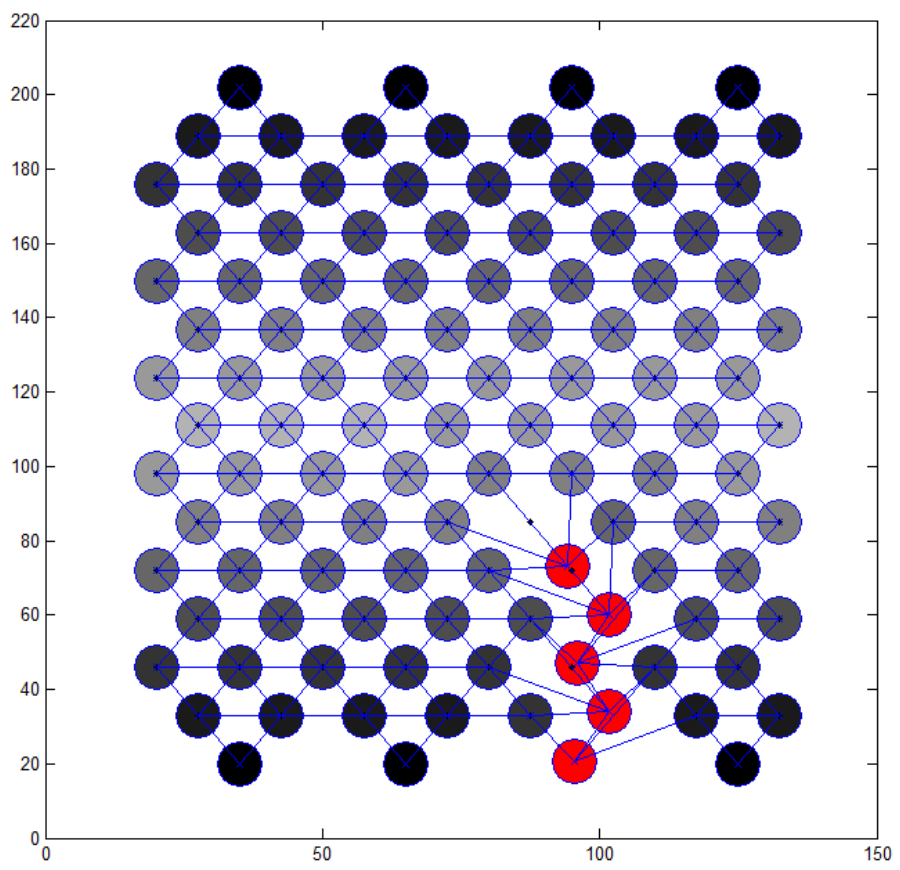
\includegraphics[width=6cm,height=6cm]{chapter5/figure5-11a.png}}
		\hspace{1cm}
		\subfigure[]{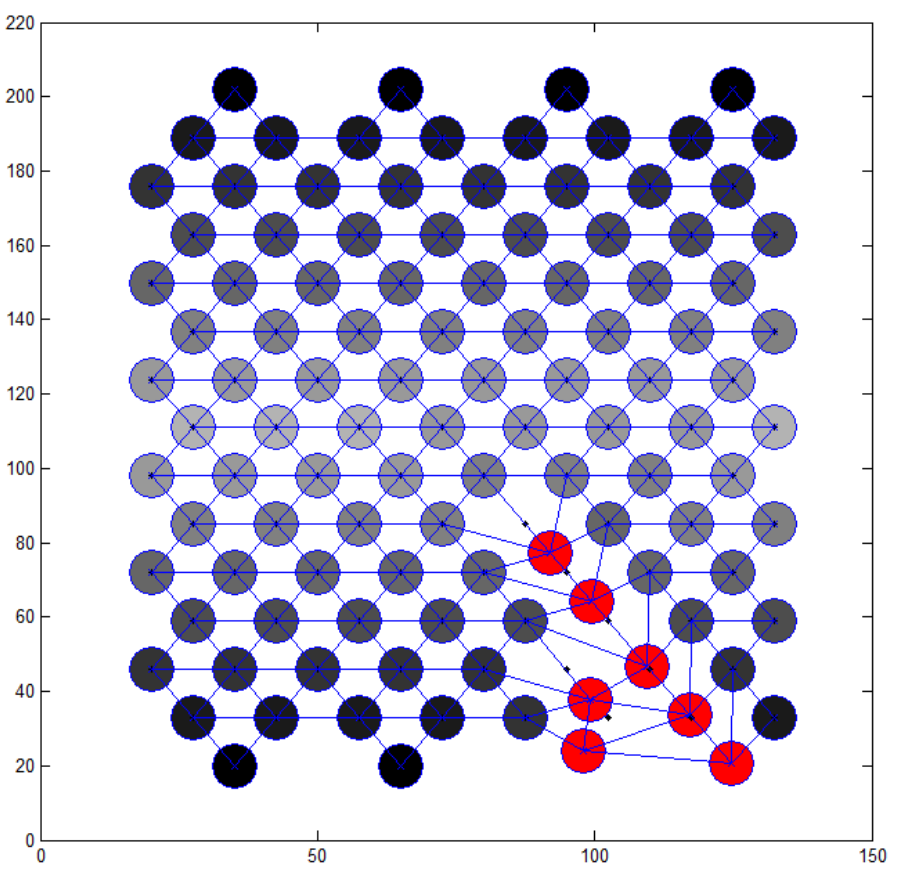
\includegraphics[width=6cm,height=6cm]{chapter5/figure5-11b.png}} \\
		\subfigure[]{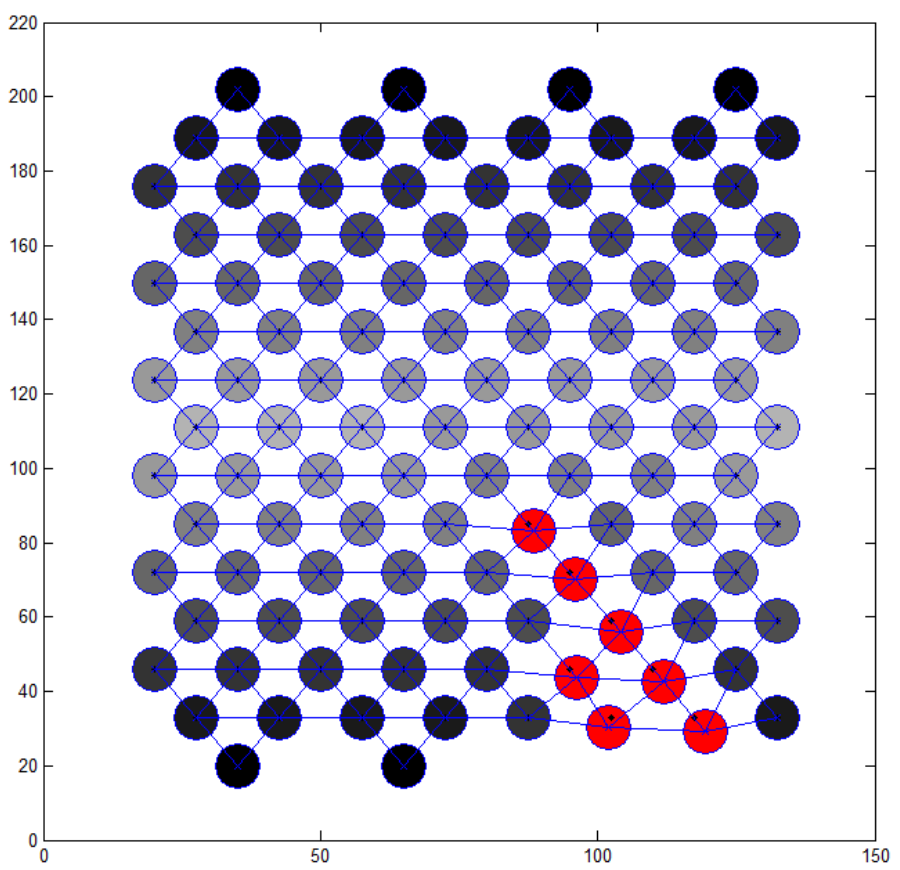
\includegraphics[width=6cm,height=6cm]{chapter5/figure5-11c.png}}
	\end{tabular}
	\bicaption[fig:repairing_robot_failed]{修复状态机器人丢失自修复过程}{修复状态机器人丢失自修复过程}{Fig}{The self-healing process of repairing robot's failure.}
\end{figure*}

\section{编队自修复实验}
本文算法在第四章介绍的自主设计的实验系统上进行了实验验证。根据实际环境与设备条件,本实验采用6台Frontier \uppercase\expandafter{\romannumeral3}型自主移动机器人,按照6邻居网络模型编成图\ref{fig:experiment_topo}所示队形,这里将机器人进行编号以方便描述。
\begin{figure}
	\centering
	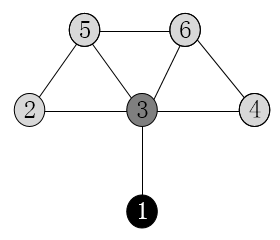
\includegraphics[width=8cm,height=7cm]{chapter5/figure5-12.png}
	\bicaption[fig:experiment_topo]{自修复实验编队模型}{自修复实验编队模型}{Fig}{The formation model of the self-healing experiment.}
\end{figure}
从图中可知,1号机器人是编队中度最小的机器人,因此根据梯度扩散规则1号机器人是梯度源节点,其他单个机器人的丢失都将由它来进行修复。在编队中2号和4号机器人是度局部极小机器人。若按照文献\parencite{liu2015gradient}中的梯度扩散规则,则2号和4号机器人也是梯度源节点并且无法得到更新。在实验中我们另5号机器人丢失,如果按照文献\parencite{liu2015gradient}的自修复规则,最终会由2号机器人进行修复,修复后的编队如图\ref{fig:local_experiment_result}所示。
\begin{figure}
	\centering
	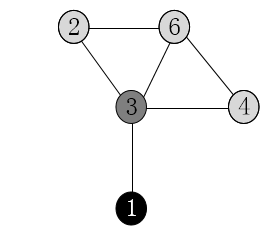
\includegraphics[width=8cm,height=7cm]{chapter5/figure5-13.png}
	\bicaption[fig:local_experiment_result]{局部最优自修复算法实验结果}{局部最优自修复算法实验结果}{Fig}{The experiment result of local optimal self-healing algorithm.}
\end{figure}

若采用本文算法,则自修复过程如图\ref{fig:global_experiment_process}所示,在5号机器人丢失后,根据竞选机制,3号机器人会竞选成功,成为第一步的修复机器人,填补5号机器人的空缺位置,5号机器人会在邻居中选取下一步的修复机器人并将修复状态传递给它。根据修复机器人选取规则,1号机器人会被选为下一步的修复机器人,填补3号机器人的空缺。1号机器人是全局度最小机器人,因此修复状态传递结束。修复完成后的编队如图\ref{fig:global_experiment_process}(d)。
\begin{figure*}
	\centering
	\subfigure[]{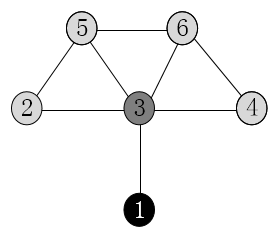
\includegraphics[width=5cm,height=4cm]{chapter5/figure5-14a.png}}
	\subfigure[]{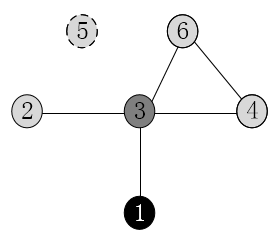
\includegraphics[width=5cm,height=4cm]{chapter5/figure5-14b.png}}
	\subfigure[]{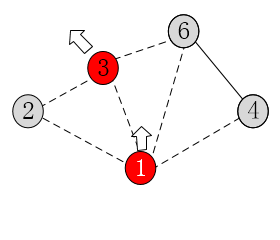
\includegraphics[width=5cm,height=4cm]{chapter5/figure5-14c.png}}
	\subfigure[]{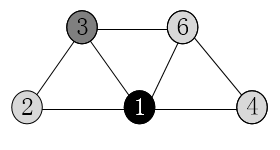
\includegraphics[width=5cm,height=4cm]{chapter5/figure5-14d.png}}
	\bicaption[fig:global_experiment_process]{全局最优自修复算法实验过程}{全局最优自修复算法实验过程}{Fig}{The experiment process of global optimal self-healing algorithm.}
\end{figure*}

图\ref{fig:real_experiment}展示了真实实验场景及过程,图中左半部分是实际Frontier \uppercase\expandafter{\romannumeral3}型自主移动机器人组成的编队队形,右半部分是在Vicon运动捕捉系统上观测到的编队图像。实验中人为取走编队中的机器人使其失效,编队能够自主的完成预期的修复效果,多次实验均能保证修复效果,证明本文算法的实际可行性和稳定性。
\begin{figure*}
	\centering
	\begin{tabular}{cc}
		\subfigure[]{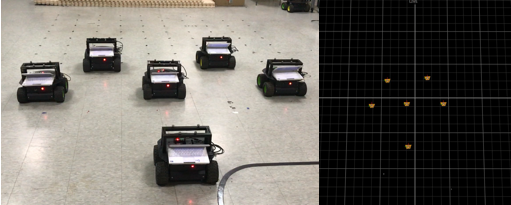
\includegraphics[width=8cm,height=4cm]{chapter5/figure5-15aaa.png}} & 
		\subfigure[]{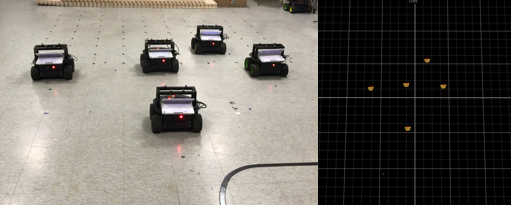
\includegraphics[width=8cm,height=4cm]{chapter5/figure5-15bbb.png}} \\
		\subfigure[]{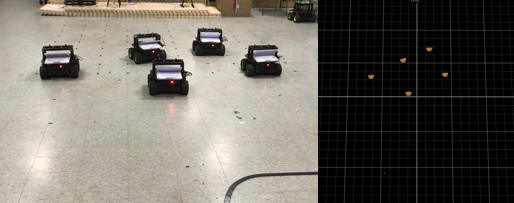
\includegraphics[width=8cm,height=4cm]{chapter5/figure5-15ccc.png}} &
		\subfigure[]{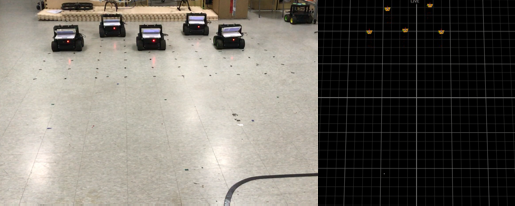
\includegraphics[width=8cm,height=4cm]{chapter5/figure5-15ddd.png}}
	\end{tabular}
	\bicaption[fig:real_experiment]{真实实验中多机器人编队的同步性改善全局最优自修复过程}{真实实验中多机器人编队的同步性改善全局最优自修复过程}{Fig}{The process of global optimal synchroniation improvement self-healing in real experiment.}
\end{figure*}

\section{本章小结}
本文主要对本文所提的同步性改善全局最优的完全分布式自修复算法进行了仿真和实验验证。仿真中将本文算法与随机自修复算法和局部最优自修复算法在同步性,修复机器人个数,修复机器人总移动距离等指标上进行了对比
。实现了本文算法在单个机器人丢失和多个机器人丢失情况下的自修复过程,同时再现了随机自修复算法和局部最优自修复算法在两种情况下的仿真。分析出随机自修复算法的随机性过大问题以及局部最优自修复算法的局部极小问题。在两种情况下的仿真结果对比中均显示出本文算法在改善同步性方面的优越性。另外还考虑了机器人在执行修复任务过程中出现缺失的自修复情况,本文算法仍然能够选出一条最优的修复路径保证同步性改善的全局最优。

在实验中,设计了6台Frontier \uppercase\expandafter{\romannumeral3}型自主移动机器人的编队场景。人为设计机器人缺失后,机器人应用本文算法能够自主进行自修复。实验中成功避开了文献\parencite{liu2015gradient}中存在的局部极小问题。多次成功实验表明本文算法的有效性和稳定性。